%% The following is a directive for TeXShop to indicate the main file
%%!TEX root = diss.tex

\chapter{An Interpretation of 3D Reconstruction}
\label{ch:3DRecon_Interp}
So far we have proposed a well-defined problem space for the 3D reconstruction problem, as well as a precise mapping from the problem space to the algorithm space. This section, we validate that the derived mapping can be reliably applied to an object with a different shape, and propose a proof-of-concept interpreter that translates the description to an appropriate algorithm that can give a reliable reconstruction result. In other words, the interpretability from the problem centric description to a reliable reconstruction result must be shown. Both synthetic and real-world datasets are provided to evaluate the performance of the interpreter.

However, such an evaluation faces several challenges. First, the mapping does not pose very strict constraints on object's geometry, and an exhaustive evaluation would require a vast number of objects to reach to a solid conclusion, which is not a practical approach. Second, we need a selection of algorithms that cover a wide range of problem space so that we can determine more convincingly if an unsuccessful result is due to lack of coverage or the limitness of the framework.

To address the first challenge, we assume \textbf{local interaction model}, which is not an uncommon assumption in vision community. Thus, geometric properties, such as concavity, that would violate this assumption will not be considered. Thus, objects with shallow concavities are used for evaluation.

For the second challenge, we need a selection of algorithms that cover a wide range of problem space. Aside from a Multi-view Stereo algorithm, we implemented a Photometric Stereo and Structured Light techniques as discussed in Chapter~\ref{ch:3DRecon_Mapping}. We can see that the selected algorithms cover a wide range of problem space, thus is sufficient to validate the framework's ability to translate the descriptive model into a reconstruction. Further, it is relatively straightforward to incorporate new algorithms, as long as they are evaluated with the same problem conditions presented in Chapter~\ref{ch:3DRecon_Mapping}. This allows researchers to contribute novel algorithms to the framework once they become available.


% In Chapter~\ref{ch:3DRecon_Mapping}, we have established a mapping from a well defined problem space to a suite of algorithms by evaluating the performance of the selected algorithms under synthetic conditions. However, the claim that this mapping would help the users obtain a satisfactory reconstruction result given the correct problem conditions is still unclear. Thus a thorough evaluation is needed to validate the proposed framework.

This chapter is organized as follows: Section~\ref{sec:interp_eval_methodology} provides a roadmap of our evaluation that is centered around two key evaluation questions: robustness of the mapping with respect to surface concavity, and robustness of the proof of concept interpeter. Section~\ref{sec:eval_mapping} investigates cases of varying surface concavity, and conditions under which the mapping can be reliably applied. Section~\ref{sec:interp} proposes a proof-of-concept interpreter, and Section~\ref{sec:eval_interp} demonstrate the robustness of the interpreter using synthetic and real-world datasets, where a satisfactory reconstruction result can be returned given the correct description of the object.

% In order to validate the 3D reconstruction mapping derived from Chapter~\ref{ch:3DRecon_Mapping}, evaluation of the object centric model into appropriate solutions must be shown. Our interpreter is based on the direct evaluation of the performance of each 3D reconstruction algorithm under different conditions presented in Chapter~\ref{ch:3DRecon_Mapping}. From this analysis of how algorithms perform on objects which have different visual and geometric properties, an algorithm(s) can be definitively chosen based on which performed best on the training images.

\section{Evaluation Methodology}
\label{sec:interp_eval_methodology}
% This section formulates the methodology of evaluation. We start with the objective, which gives a brief introduction of what needs to be evaluated. Next, two key evaluation questions are proposed, with evaluation steps, criteria and expected outcomes to determine if the evaluation is successful.

% \subsection{Objective}
% [Develop a description (or access an existing version) of what is to be evaluated and how it is understood to work.]
This evaluation intends to 1) validate that the mapping from Chapter~\ref{ch:3DRecon_Mapping} can be extended to objects with different shapes, and demonstrate cases where it succeeds and fails; and 2) demonstrate the robustness of the proof-of-concept interpreter using synthetic and real-world datasets. For our first goal, objects with varied degrees of shape (concavity) changes are used, and the corresponding results are compared to the mapping. We attempt to demonstrate if the mapping, to some extent, is robust to the changes of shape, and when it would fail to hold. For the second goal, we use synthetic and real-world objects to demonstrate that the interpreter can return a satisfactory result when provided with a correct description.

% \subsection{Frame}
% Set the parameters of the evaluation its purposes, key evaluation questions and the criteria and standards to be used.

% \subsubsection{Purpose}
% [What are the primary purposes and intended uses of the evaluation?]
% The evaluation intends to find out that the derived mapping can indeed find the algorithm that produces the best possible result from a suite of algorithms.

\subsection{Key Evaluation Questions and Steps}
% [What are the high level questions the evaluation will seek to answer? How can these be developed?]

The evaluation attempts to \textit{prove that the mapping can be extended to other objects with different geometries}, and \textit{demonstrate that the framework can return a satisfactory reconstruction result given a correct description}.

\subsubsection{1. Is the mapping robust to changes of object's shape?}
We first need to verify that the mapping derived in Chapter~\ref{ch:3DRecon_Mapping} is applicable to objects with different shapes. The variation of geometry is too vast and complicated to model, so it wouldn't be possible to consider all possible conditions. As mentioned before, we focus on one geometric property, surface concavity, that in theory can have an impact on the results. We use three synthetic objects with varied degrees of concavity, and verify if the mapping is applicable under all circumstances, and when it would succeed or fail. We use synthetic data to verify the mapping since it would not be practical to change material properties using real world objects. The details of evaluation include:

% \noindent\textbf{System setup}: the synthetic data is generated by the Blender using the same setups in Chapter~\ref{ch:3DRecon_Mapping};

\noindent\textbf{Data generation} the synthetic data is generated in Blender using the same setups presented in Chapter~\ref{ch:3DRecon_Mapping}. We consider the four property settings that represent four major classes of real-world objects from Chapter~\ref{ch:3DRecon_Taxo}.

% \noindent\textbf{Algorithm execution and evaluation}: three selected algorithms as well as the baseline are used to reconstruct the synthetic object. Quantitative and qualitative results are plotted;

\noindent\textbf{Validation} consisting of two steps: 1) the successful algorithm(s) in each case need be identified based on qualitative and quantitative results; 2) the reliable algorithms in each case should be consistent with the mapping results. If that is not the case, we need to find out how robust each algorithm in within the mapping is with respect to concavity changes, and how concavity change affects the reconstruction results.

\noindent\textbf{Criteria} To determine that a method returns a reliable result, the accuracy value should be lower than that of the baseline method while the completeness should be higher, and all the statistical measures of the angular error must also be lower than those of the baseline method, including the mean, median, standard deviation, and interquartile range. The qualitative results are used to further confirm the validity of the quantitative results and give a visual sense of the cause of failed reconstruction.

\subsubsection{2. Can the proof-of-concept interpreter return a satisfactory reconstruction given the correct description?}
Given a correct description of an object, the algorithm chosen by the proof-of-concept interpreter should give a satisfactory reconstruction result of a real-world object. In this case, visual inspection is utilized to determine the quality of reconstruction results since ground true data is unavailable, thus quantitative results cannot be computed. The framework would use the algorithm determined by mapping for reconstruction, the result of which would then compared to the baseline algorithm to determine if the quality is acceptable. As previously mentioned, the baseline method is chosen so that it can always provide a decent reconstruction under most circumstances. The details of evaluation are presented as follows:

\noindent\textbf{Data generation}: real-world data are captured using similar setups as the synthetic counterparts: for MVS, a Nikon D70S camera with a $18-70mm$ lens are used; for photometric images, a Nikon D70S camera with a $70-200mm$ lens, a handheld lamp, and two reference objects are used (diffuse and glossy); for structured light techniques, a Nikon 70S camera and a Sanyo Pro xtraX Multiverse projector are used, which is positioned with a between angle of around $10^\circ$. We used nine everyday objects with varying textures, reflectance properties, and shapes with low concavity.

\noindent\textbf{Validation}: we need to demonstrate that the interpreter would return a reliable reconstructed model given the correct description, and a less successful model given an invalid description. The quality of the reconstruction is determined by comparing the result to the baseline method.
% Second, the algorithm chosen by the interpreter should be one of the top performers among all the algorithms implemented within the framework.

\noindent\textbf{Output}: the output of Photometric Stereo algorithms, typically a normal map, is integrated to a surface mesh for visual inspection.

% \subsubsection{2. Usefulness of Mapping: How the mapping will return the result based on your description and your requirements}
% The purpose of the framework is not to compare which algorithm gives the best result, but to get the best possible reconstruction result given the correct description. Therefore, we want to see how well it works given the correct description, and how badly the result deteriorates given the incorrect description.

% The evaluation steps are:
% \begin{itemize}
% \item We chose three objects so that each algorithm would be activated by the mapping once as a demonstrative result.
% \item 
% \end{itemize}

% \subsubsection{2. Robustness: Does the mapping still return the best algorithm given an incorrect description?}
% Assume given a incorrect description of the object, will the mapping return a less satisfactory result instead, which is what it should behave like?

% \subsubsection{3. Improvement: Is the mapping more useful than the traditional approach?}
% Aside from being able to get the correct results, it's also important that the proposed approach has significant advantages over the traditional ones. We first need to identify the traditional way of employing reconstruction algorithms, find out the strengths and weakness and see if the proposed approach is superior than the exising one in the claimed aspects. The following are the aspects we set out to compare:
% \begin{itemize}
% \item is it easier?
% \item does it cater to more general object?
% \end{itemize}

% The evaluation steps are:
% \begin{itemize}
% \item Define the fundamental steps for both the traditional approach and the one proposed in the thesis.
% \item we adopt the same approach for analysing algorithmic complexity, and use basic step as the unit step to evaluate the complexity of using these two approaches. Complexity analysis is also a tool that allows us to explain how an algorithm behaves as the input grows larger. fundamental instructions/steps
% \end{itemize}

% \subsubsection{Criteria}
% Determine what `success' look like? What should be the criteria and standards for judging performance? Whose criteria and standards matter? What process should be used to develop agreement about these?

% \subsubsection{Steps}
% [Collect and retrieve data to answer descriptive questions about the activities of the project/programme/policy, the various results it has had, and the context in which it has been implemented.]

\section{Parameter Setting}
The first step of using the framework is to estimate the parameters of an object's properties. We use the BRDF explorer developed by Disney Animation~\cite{disnybrdf} to visualize the rendered object with changing properties. A ``try-and-see'' approach was taken to obtain the parameters. More specifically, the user would change the value of each property and see if the rendered result looks like the real object. A similar approach can be found in~\cite{Berkiten:2016:ARB} where \citeauthor{Berkiten:2016:ARB} also use a synthetic dataset to find the contributing factors of various Photometric Stereo algorithms.
\begin{figure}[!htbp]
\centering
\begin{tabular}{cc}
  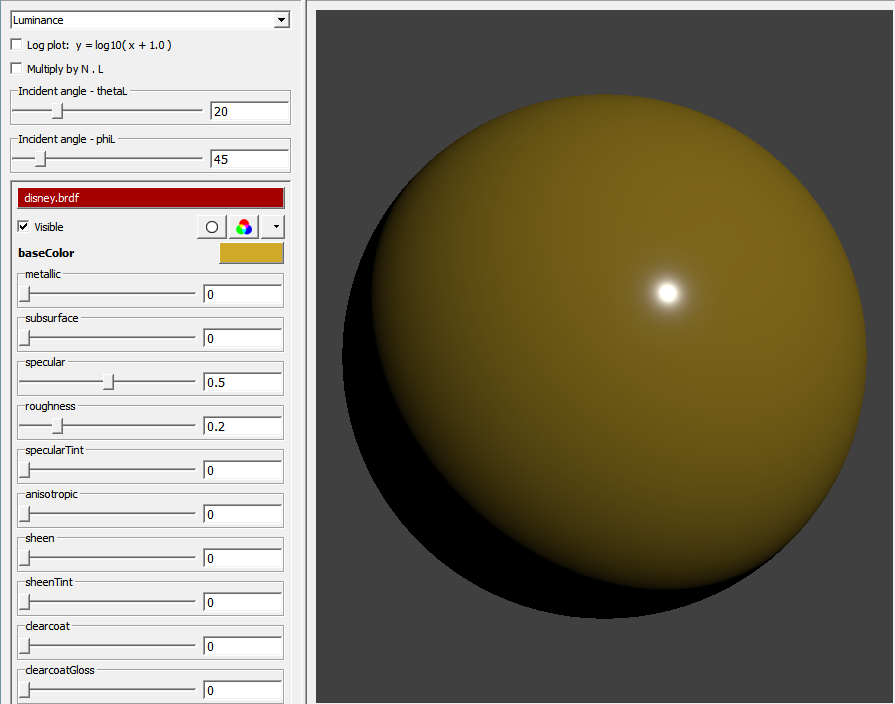
\includegraphics[width=0.4\textwidth]{interp/ui_sphere.PNG}&
  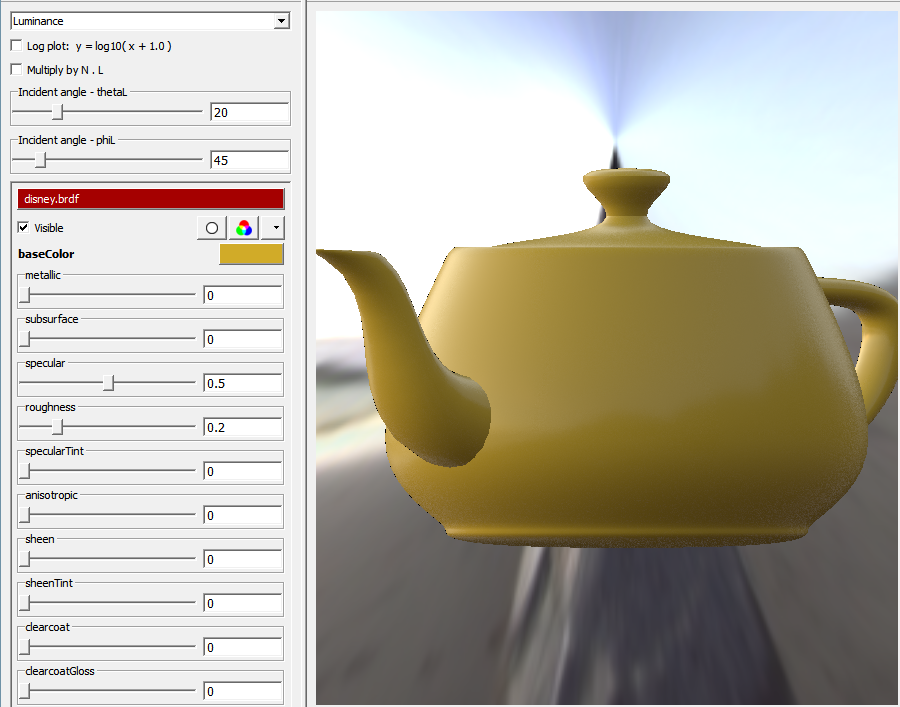
\includegraphics[width=0.4\textwidth]{interp/ui_teapot.PNG}\\
  (a) Lit sphere & (b) Lit teapot\\
\end{tabular}
\caption{The UI for determining the property settings, including albedo, specular, and roughness of the surface. The albedo is set as the value channel of HSV colour space. In this case, the albedo is set as 0.8, and the specular and roughness is set as 0.5, 0.2, respectively. (a) demonstrates the effect of the property settings on a sphere while (b) on a teapot.}
\label{fig:ui}
\end{figure}

\section{Evaluation of Mapping}
\label{sec:eval_mapping}
We first validate that the derived mapping can be applied to an object with a different shape. Given the description of an arbitrary object, we wish to use all three techniques for reconstruction, to see if the algorithm that has the best quantitative or qualitative results is consistent to the algorithm chosen by the mapping.

\subsection{Synthetic Datasets}
We use three objects with increasing degree of concavity, which are `bottle', `knight', and `king', as shown in Figure~\ref{fig:synth_data}. We select four property settings representing the four classes of the most commonly seen objects discussed in Chapter~\ref{ch:3DRecon_Desc}, which is shown in Table~\ref{tab:prop_list_synth_data} to assess the robustness of the mapping. We present the results of the mapping in Table~\ref{tab:prop_list_synth_data} as a reference to check if the quantitative and qualitative results from the testing data is consistent with the results of the mapping. The results are shown in Figure~\ref{fig:synth_data_results_bottle},~\ref{fig:synth_data_results_knight}, and~\ref{fig:synth_data_results_king}.
\begin{table}[!htbp]
  \centering
  \begin{tabular}{*{3}{p{8mm}}*{2}{p{15mm}}|*{3}{r}}
  \hline
  & & & & & \multicolumn{3}{c}{Metrics}\\
  Class & Texture & Albedo & Specularity & Roughness & Accuracy & Completeness & Ang error\\
  \hline
  (a) & 0.2 & 0.8 & 0.2 & 0.8 & GSL & GSL & EPS\\
  (b) & 0.2 & 0.8 & 0.5 & 0.2 & GSL & - & - \\
  (c) & 0.8 & 0.8 & 0.2 & 0.8 & PMVS, GSL & PMVS, GSL & EPS \\
  (d) & 0.8 & 0.8 & 0.5 & 0.2 & PMVS, GSL & PMVS & -\\
  \hline
  \end{tabular}
  \caption{Property settings of the three testing objects: `bottle', `knight', `king', which have increasing degree of concavity.}
  \label{tab:prop_list_synth_data}
\end{table}

\begin{figure}[!htbp]
\centering
\begin{tabular}{cccc}
  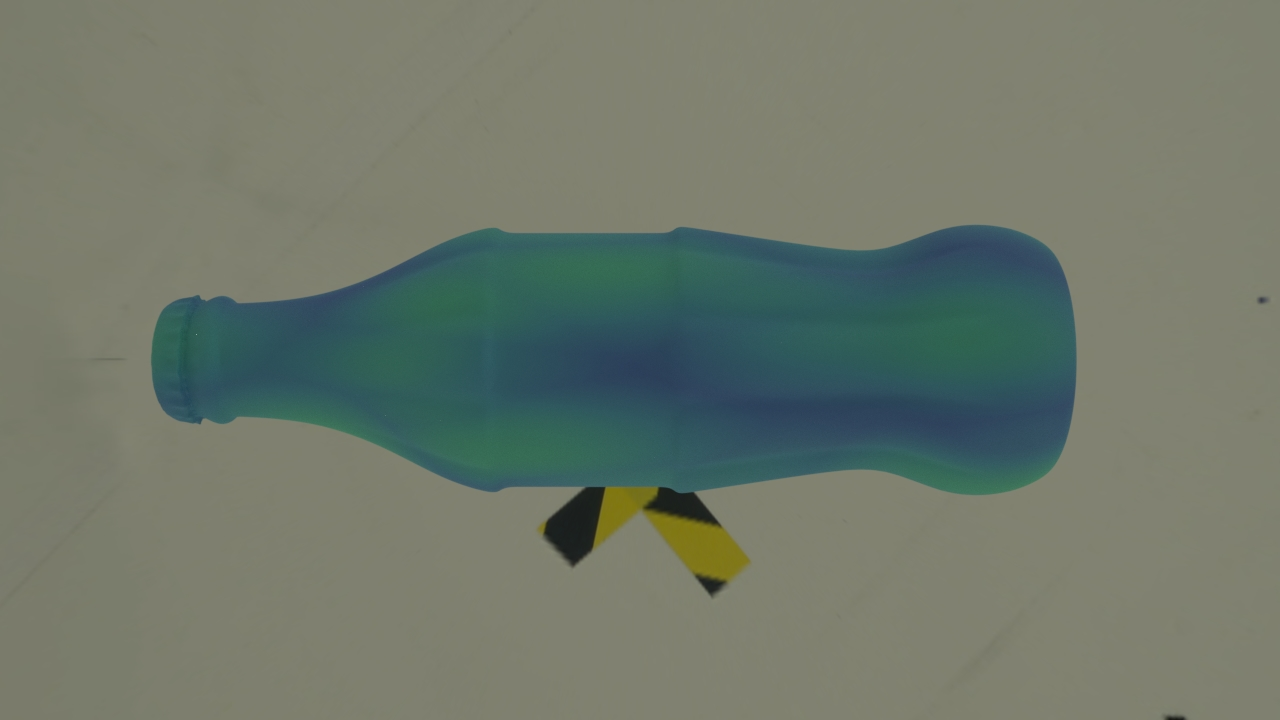
\includegraphics[width=0.2\textwidth]{interp/synth_data/bottle/bottle_mvs}&
  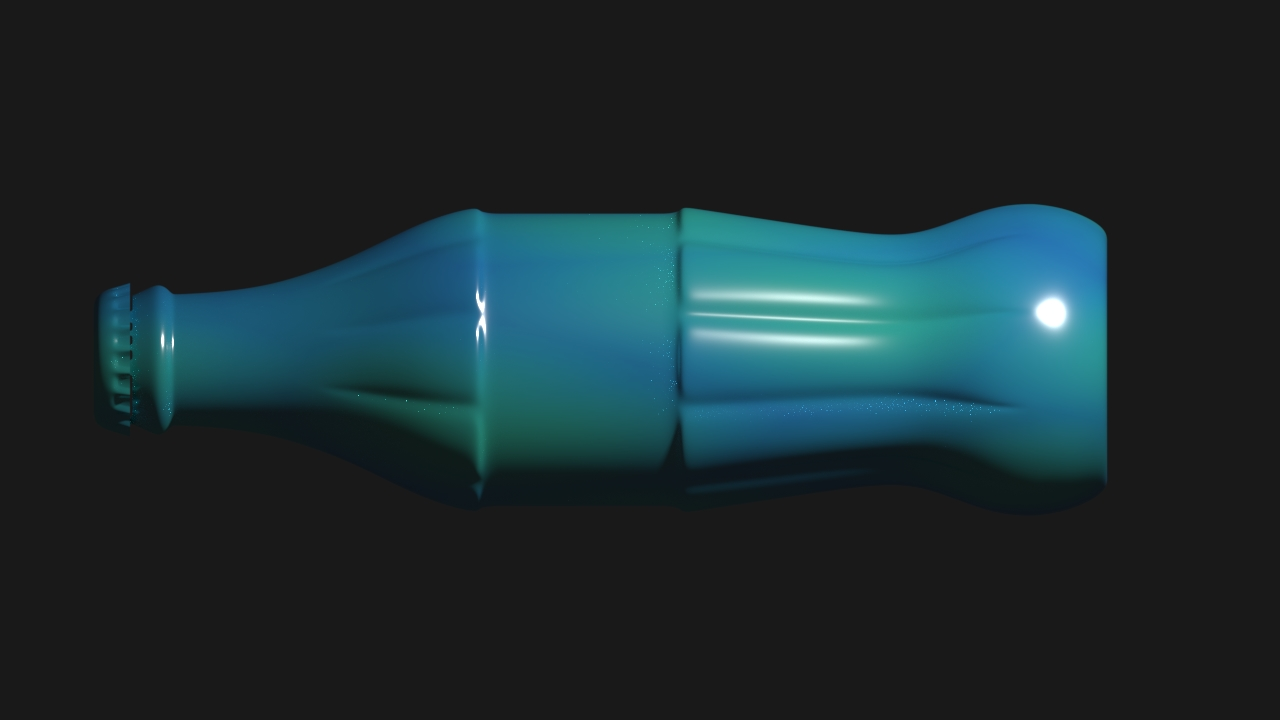
\includegraphics[width=0.2\textwidth]{interp/synth_data/bottle/bottle_ps}&
  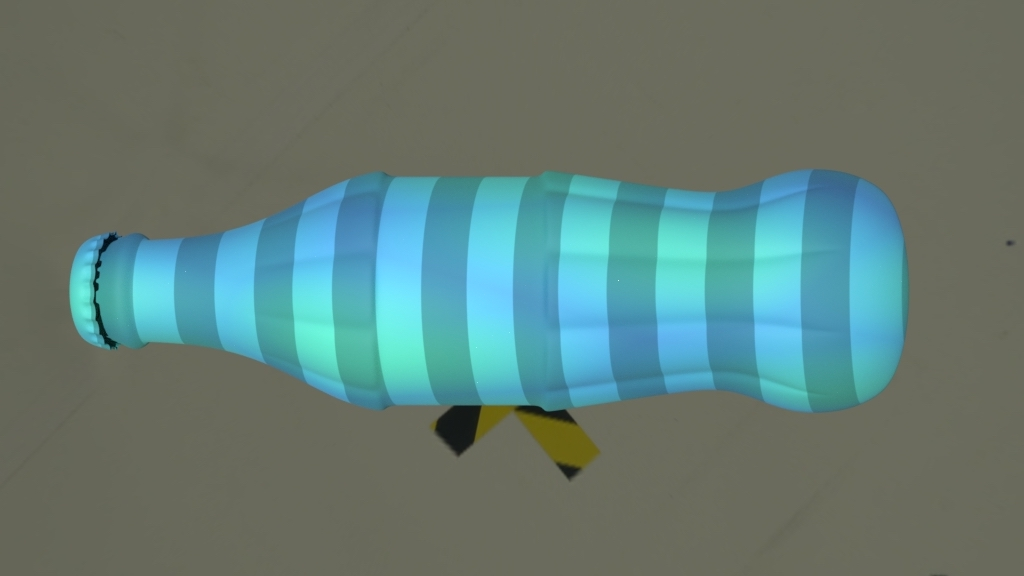
\includegraphics[width=0.2\textwidth]{interp/synth_data/bottle/bottle_sl}&
  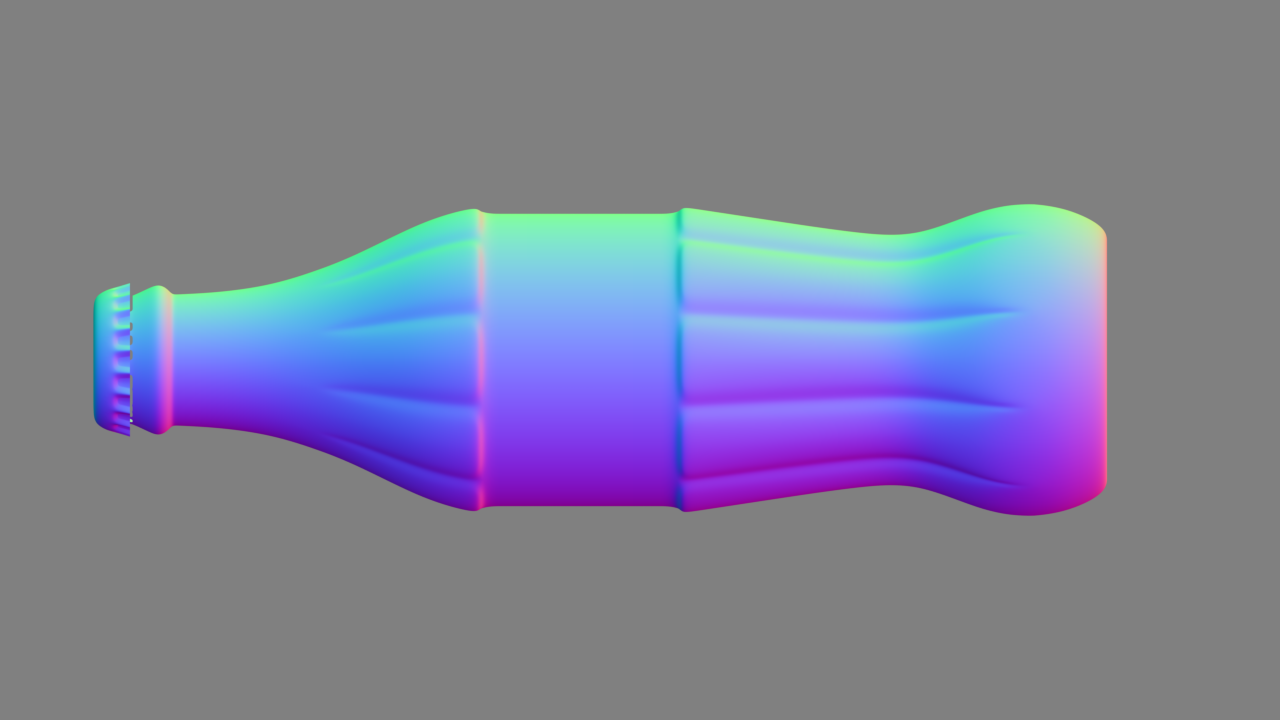
\includegraphics[width=0.2\textwidth]{interp/synth_data/bottle/bottle_ps_gt}\\
  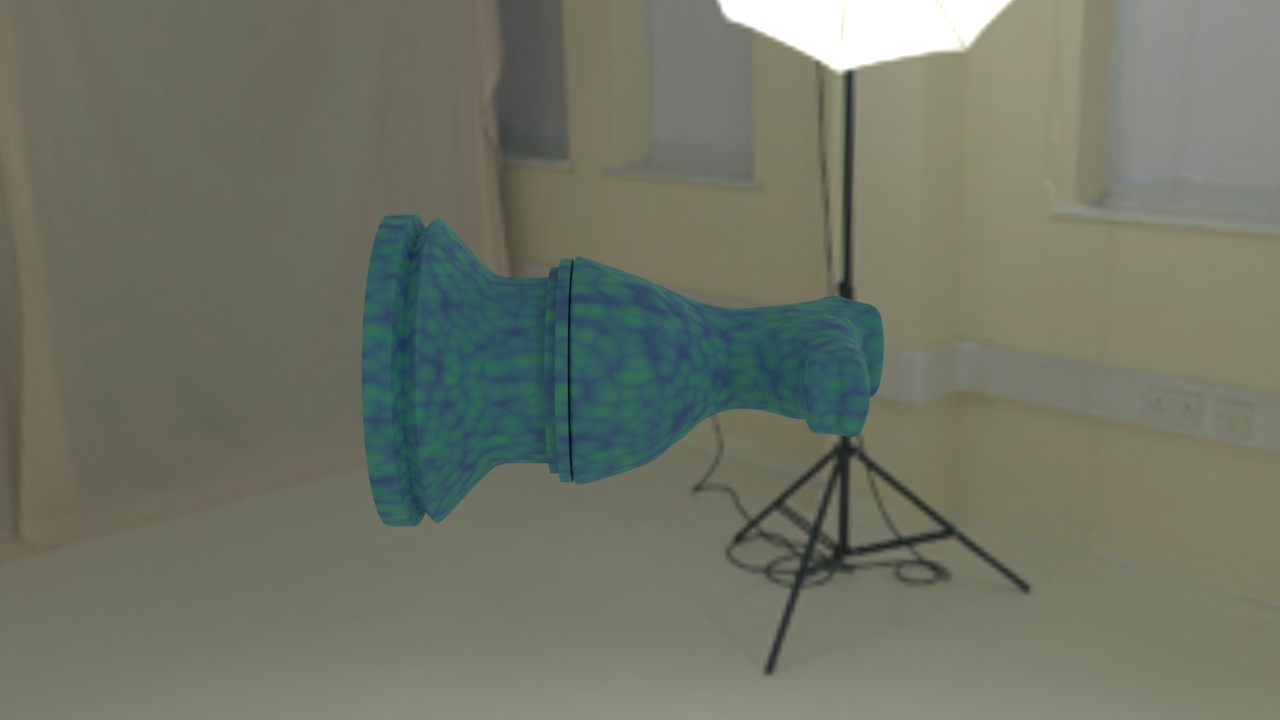
\includegraphics[width=0.2\textwidth]{interp/synth_data/knight/knight_mvs}&
  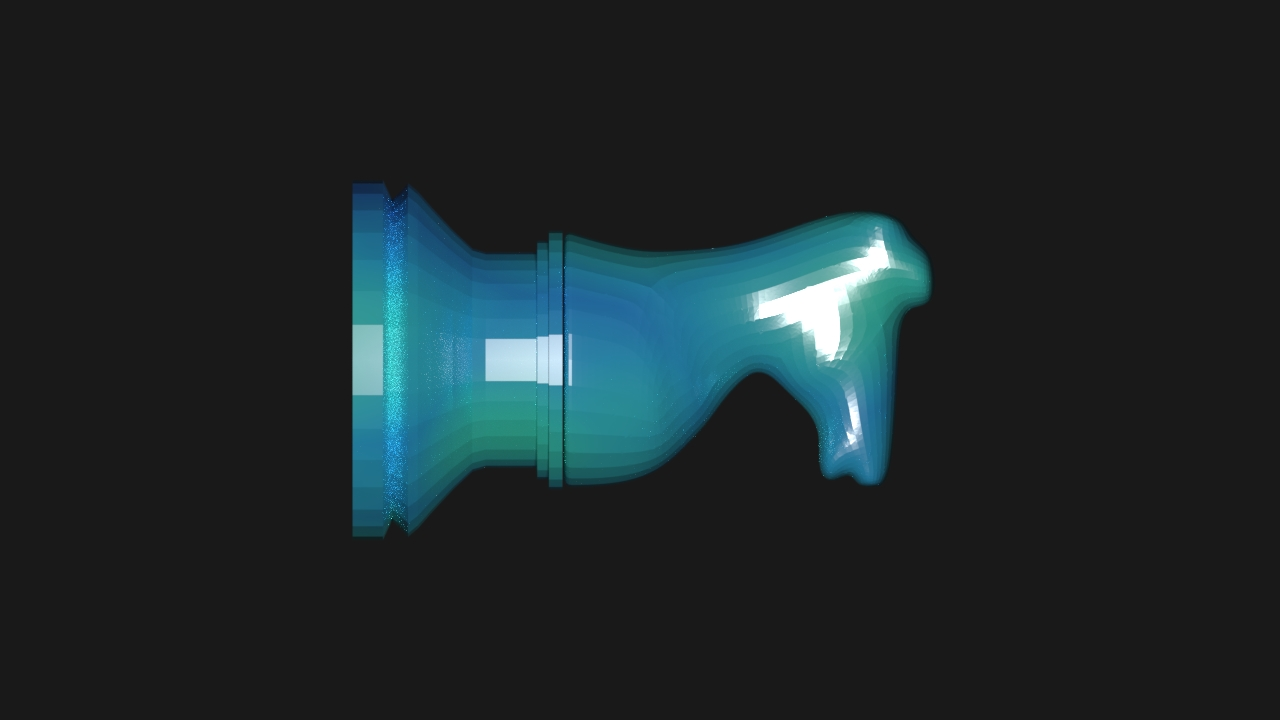
\includegraphics[width=0.2\textwidth]{interp/synth_data/knight/knight_ps}&
  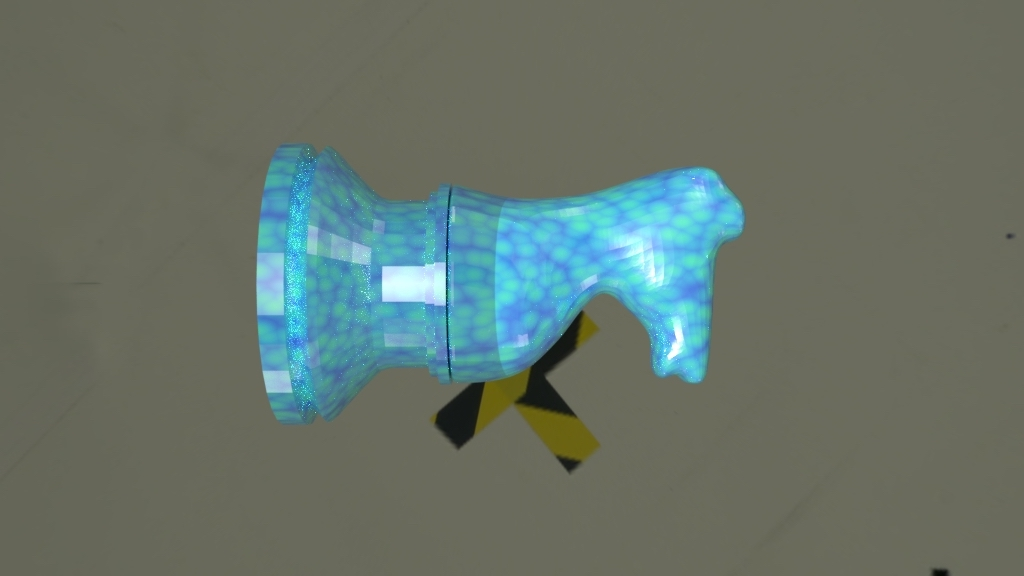
\includegraphics[width=0.2\textwidth]{interp/synth_data/knight/knight_sl}&
  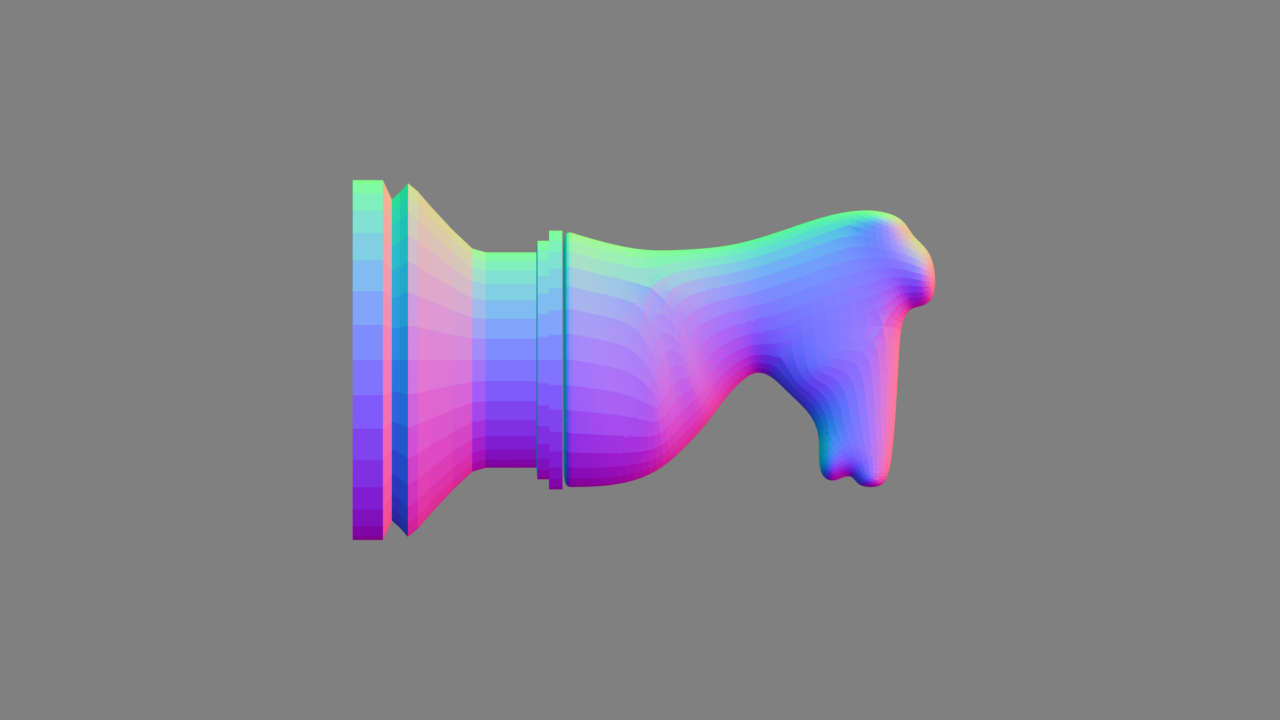
\includegraphics[width=0.2\textwidth]{interp/synth_data/knight/knight_ps_gt}\\
  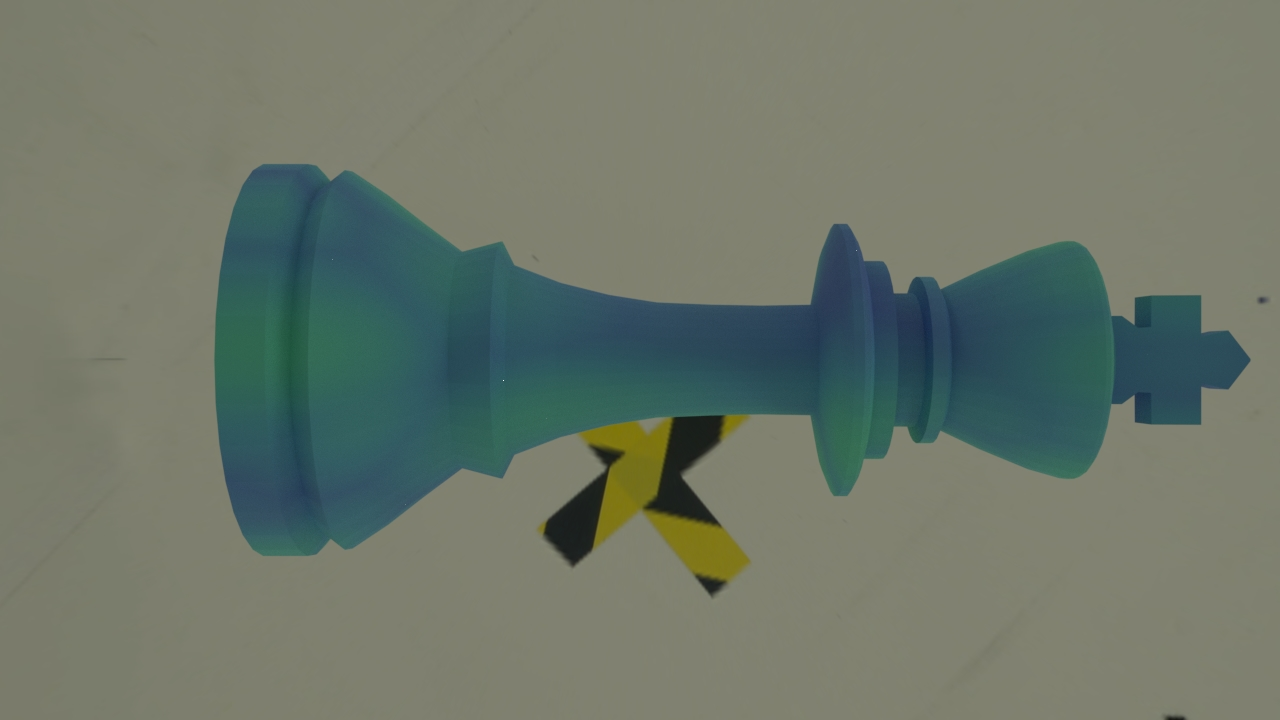
\includegraphics[width=0.2\textwidth]{interp/synth_data/king/king_mvs}&
  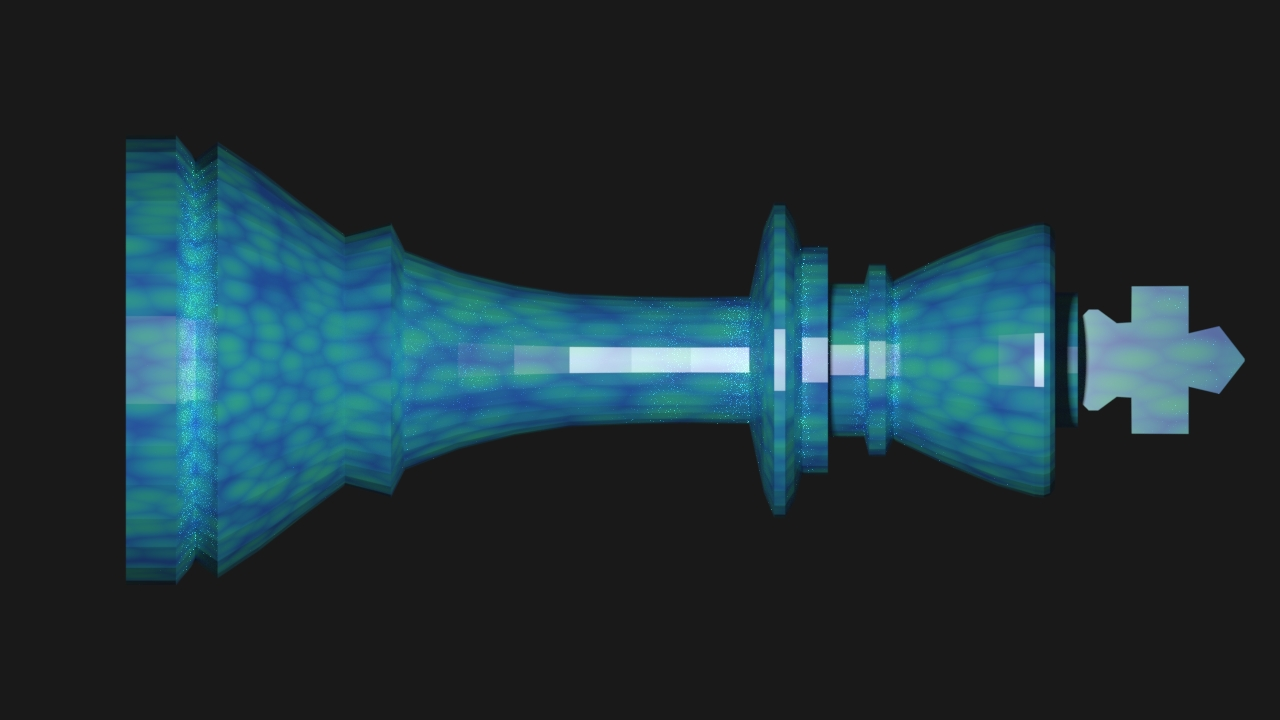
\includegraphics[width=0.2\textwidth]{interp/synth_data/king/king_ps}&
  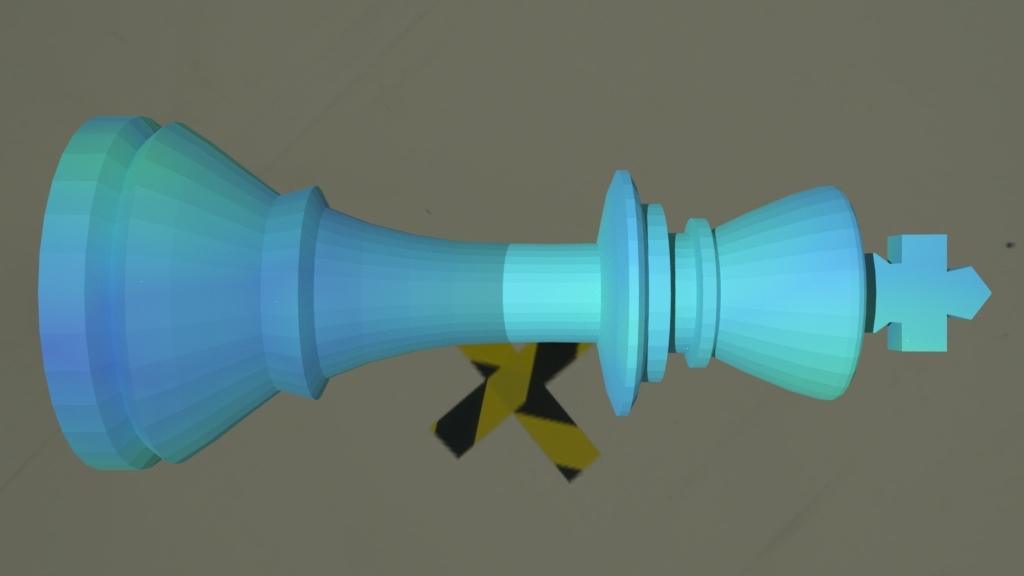
\includegraphics[width=0.2\textwidth]{interp/synth_data/king/king_sl}&
  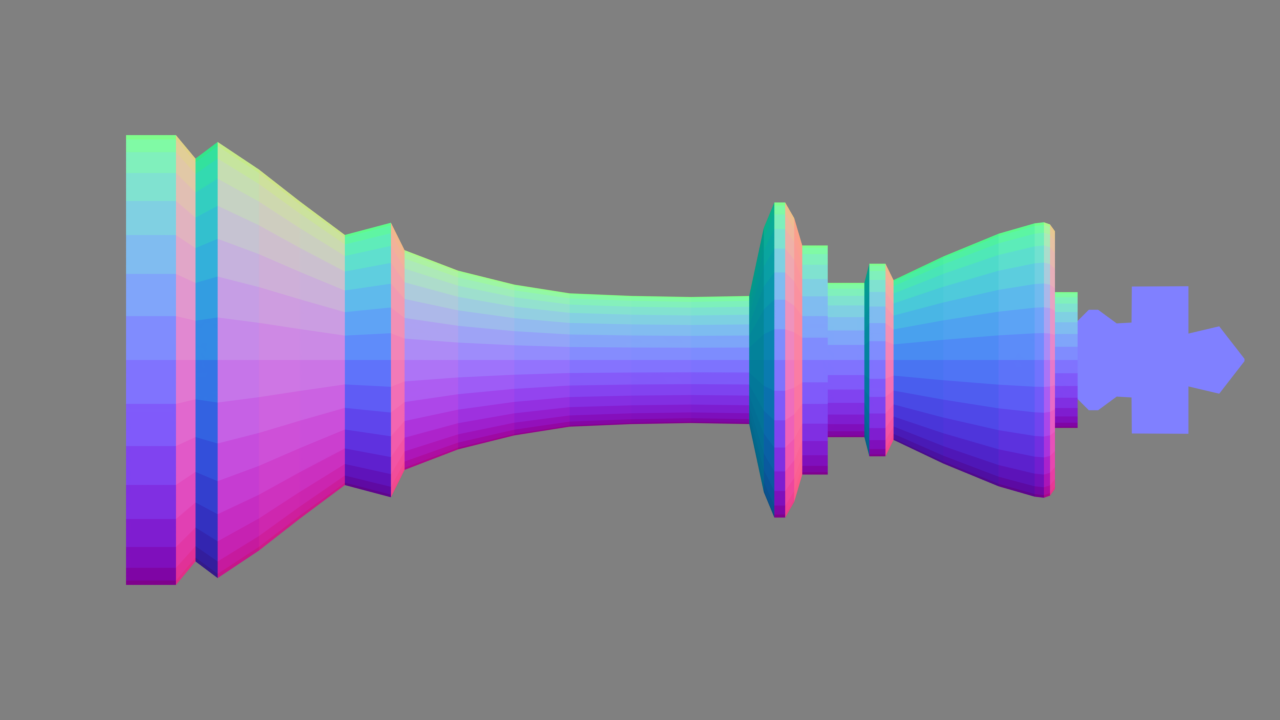
\includegraphics[width=0.2\textwidth]{interp/synth_data/king/king_ps_gt}\\
  MVS & PS & SL & Normal groundtruth\\
\end{tabular}
\caption{The synthetic dataset and groundtruth for the evaluation of the robustness of the mapping to concavity. Three objects with varied degrees of concavity are selected, each is configured with four properties settings listed in Table~\ref{tab:prop_list_synth_data}.}
\label{fig:synth_data}
\end{figure}

% Here is the Table to test the effectiveness of the mapping
% \begin{figure}[!htbp]
% \centering
% \begin{tabular}{cccccc}
% \hline
% & & Mapping & \multicolumn{2}{c}{Accu\&Cmplt} & Norm\\
% \hline
% \multirow{2}{*}{Obj} & \multirow{2}{*}{Desc} & \multirow{2}{*}{Algo} & PMVS & Gray SL & Example PS\\
% 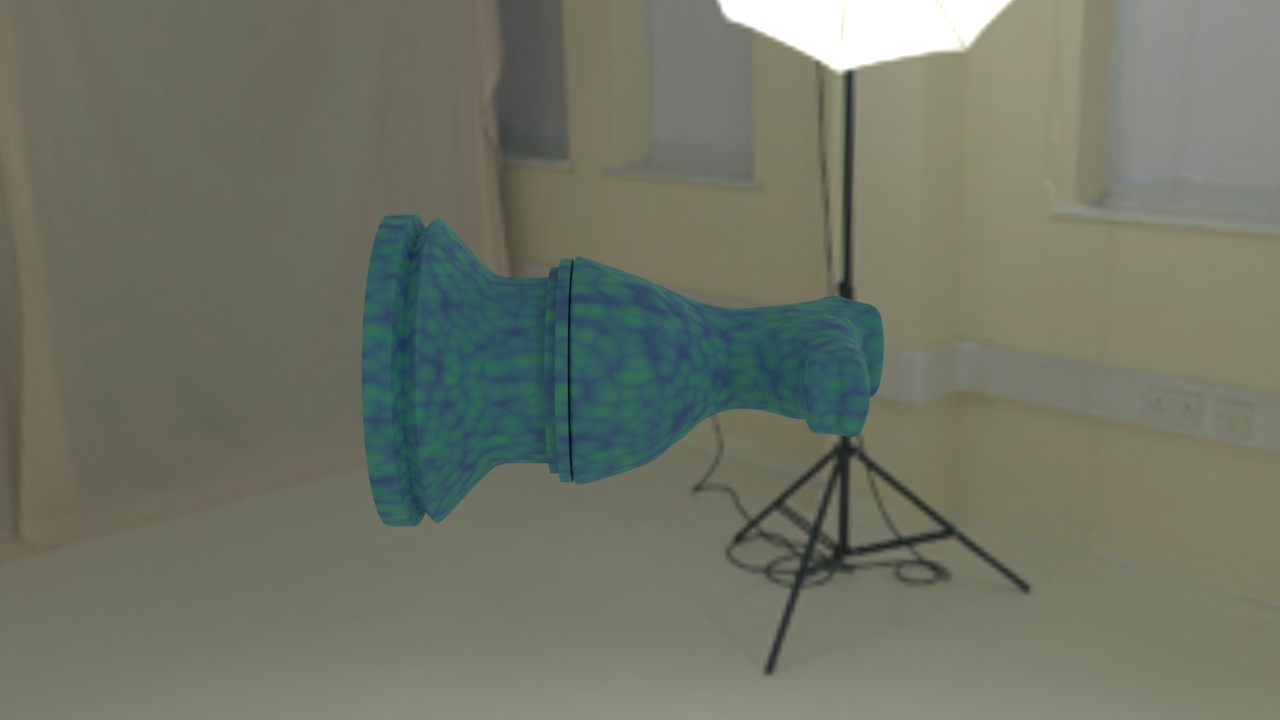
\includegraphics[width=0.15\textwidth]{interp/synth_data/knight/knight_mvs} &
% 02080208 & EPS, GSL & 
% 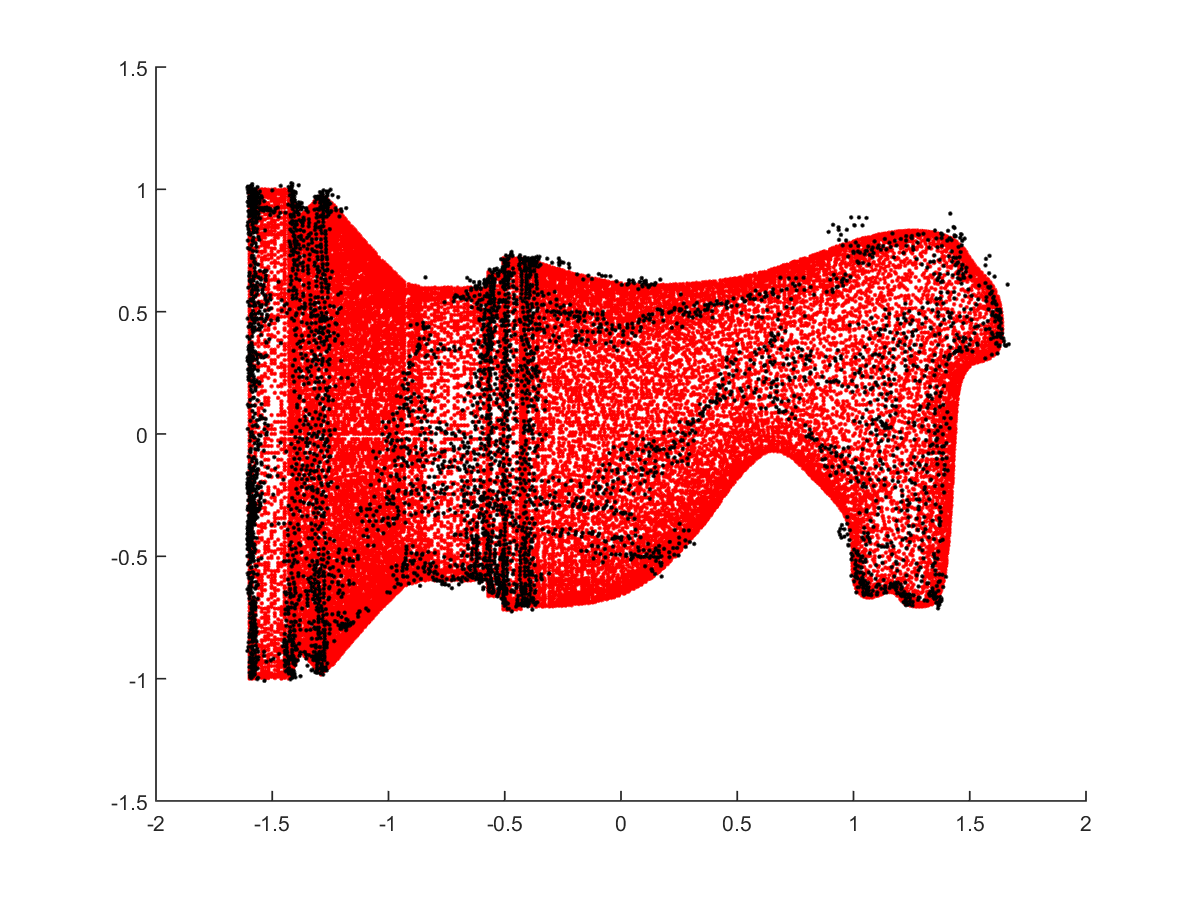
\includegraphics[width=0.15\textwidth]{interp/synth_data/knight/knight_mvs_02080208} &
% 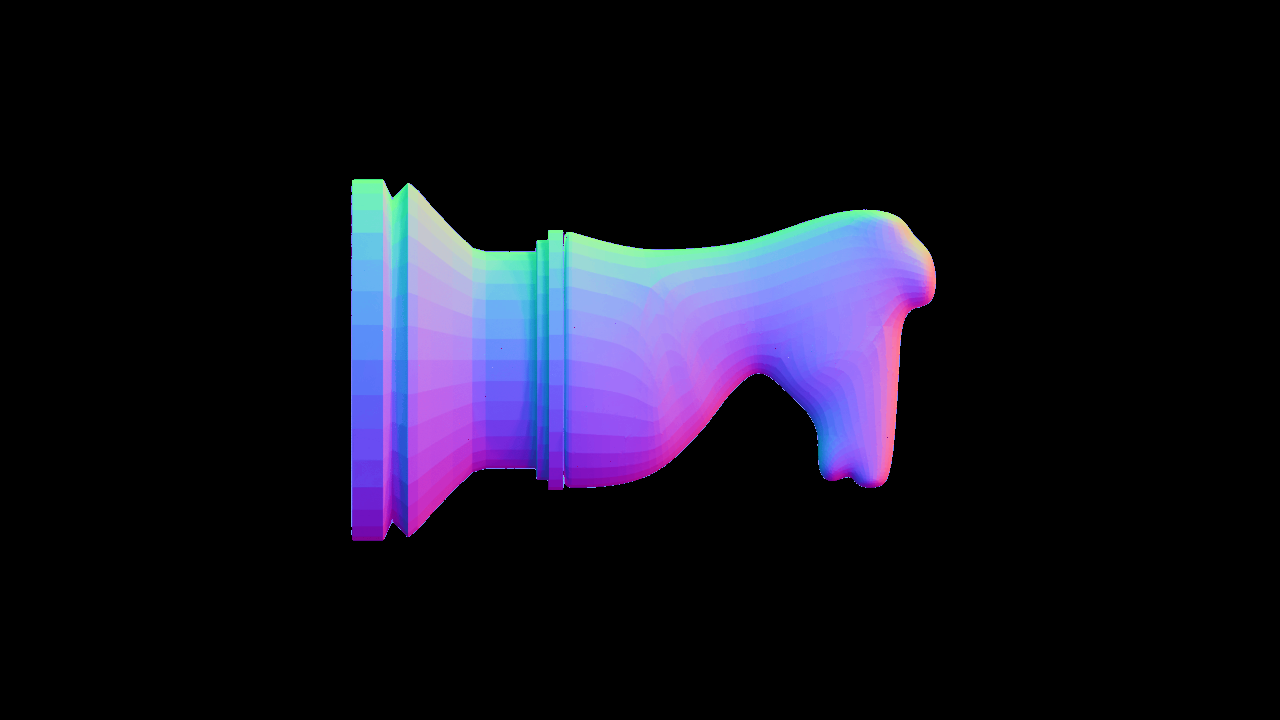
\includegraphics[width=0.15\textwidth]{interp/synth_data/knight/knight_ps_02080208} &
% 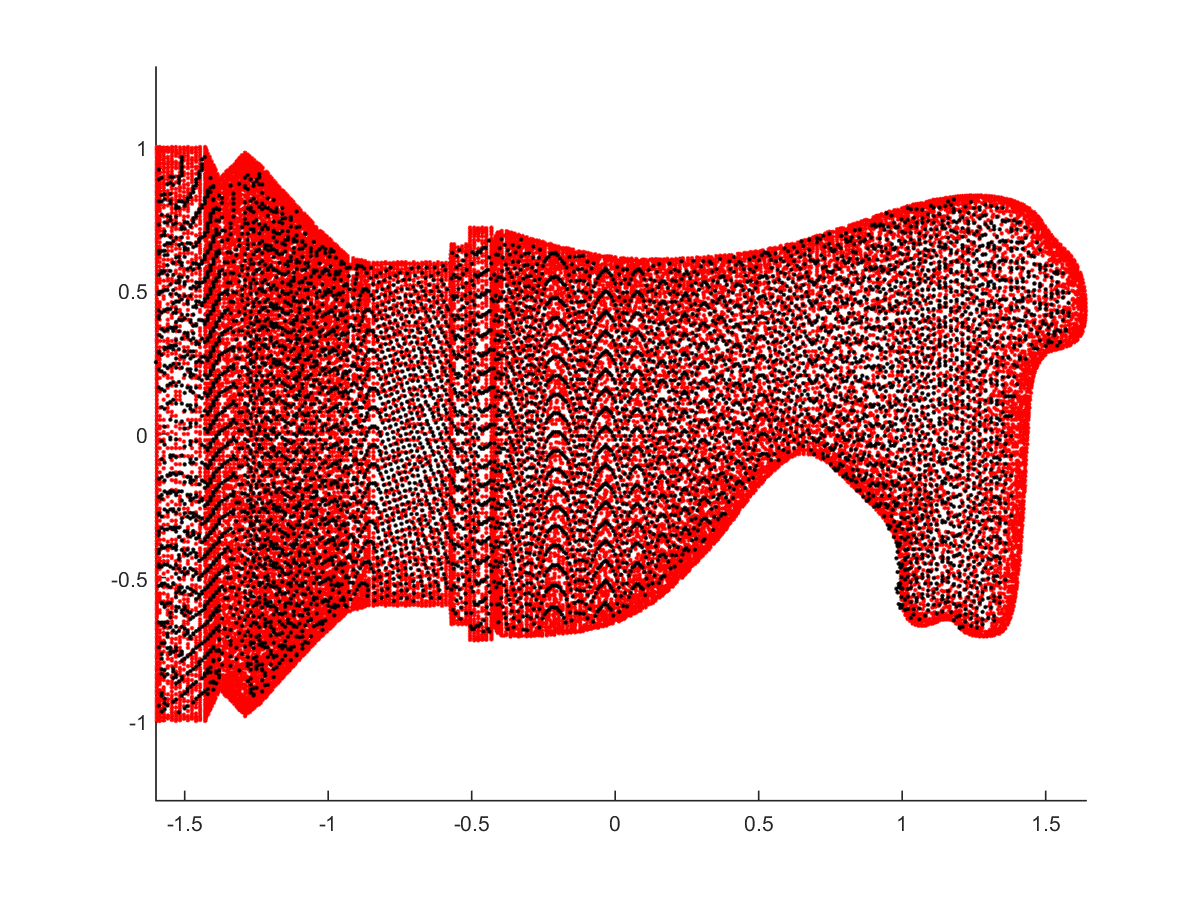
\includegraphics[width=0.15\textwidth]{interp/synth_data/knight/knight_sl_02080208}\\
% \hline
% \end{tabular}
% \end{figure}

\subsubsection{Data 1: bottle}
The first test object is a `bottle', which has shallow indentations on the surface, \ie low level concavity. The synthetic object is configured with the four property settings listed in Table~\ref{tab:prop_list_synth_data}. The first column presents the results of the mapping, and the algorithms that produce acceptable results are labeled in the green box. All quantitative and qualitative results align with those of the mapping, so we claim that the mapping is successfully applied to a surface with low concavity.
\begin{sidewaysfigure}[!htbp]
\centering
\begin{tabular}{c|ccccc}
  Mapping & Quantitative results & ~ & Qualitative results & ~\\
  \hline
  EPS, GSL & 
  \includegraphics[width=0.2\textwidth]{interp/synth_data/bottle/bottle_02080208}&
  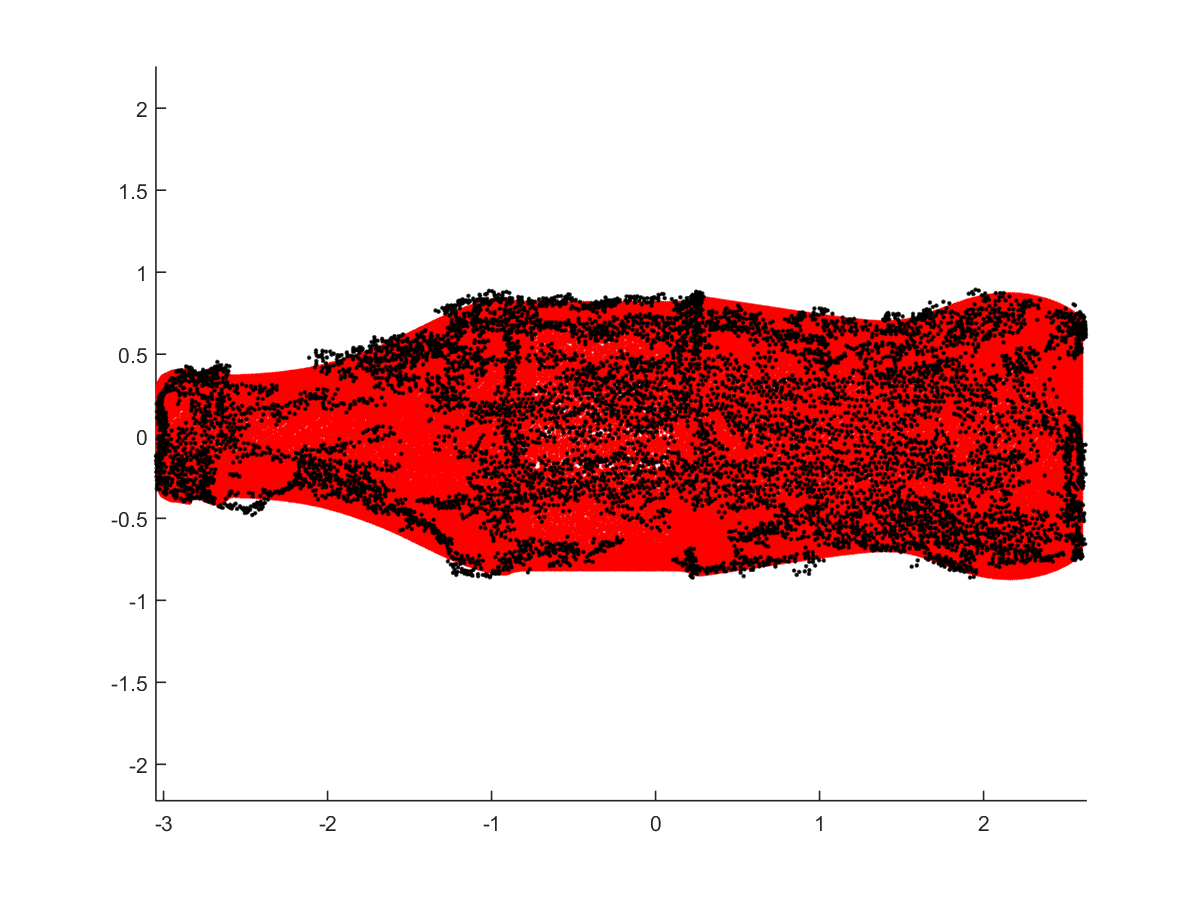
\includegraphics[width=0.2\textwidth]{interp/synth_data/bottle/bottle_mvs_02080208.png}&
  \fcolorbox{green}{white}{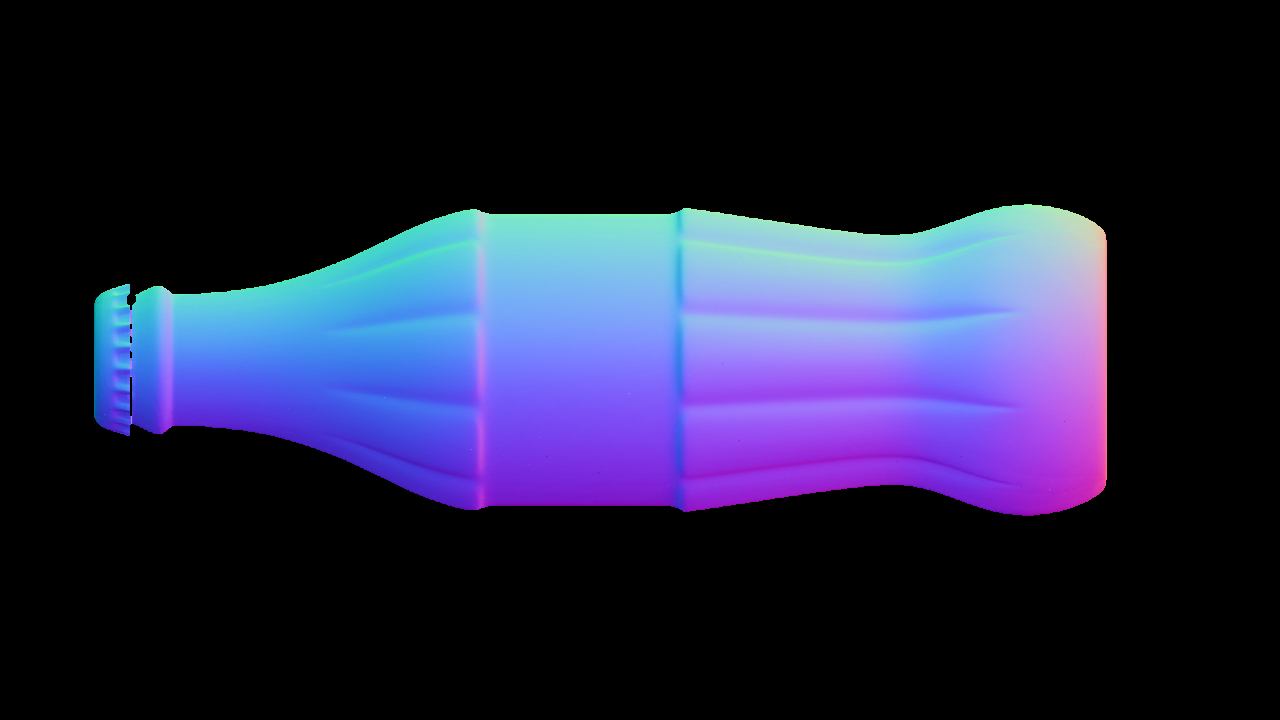
\includegraphics[width=0.2\textwidth]{interp/synth_data/bottle/bottle_ps_02080208.png}}&
  \fcolorbox{green}{white}{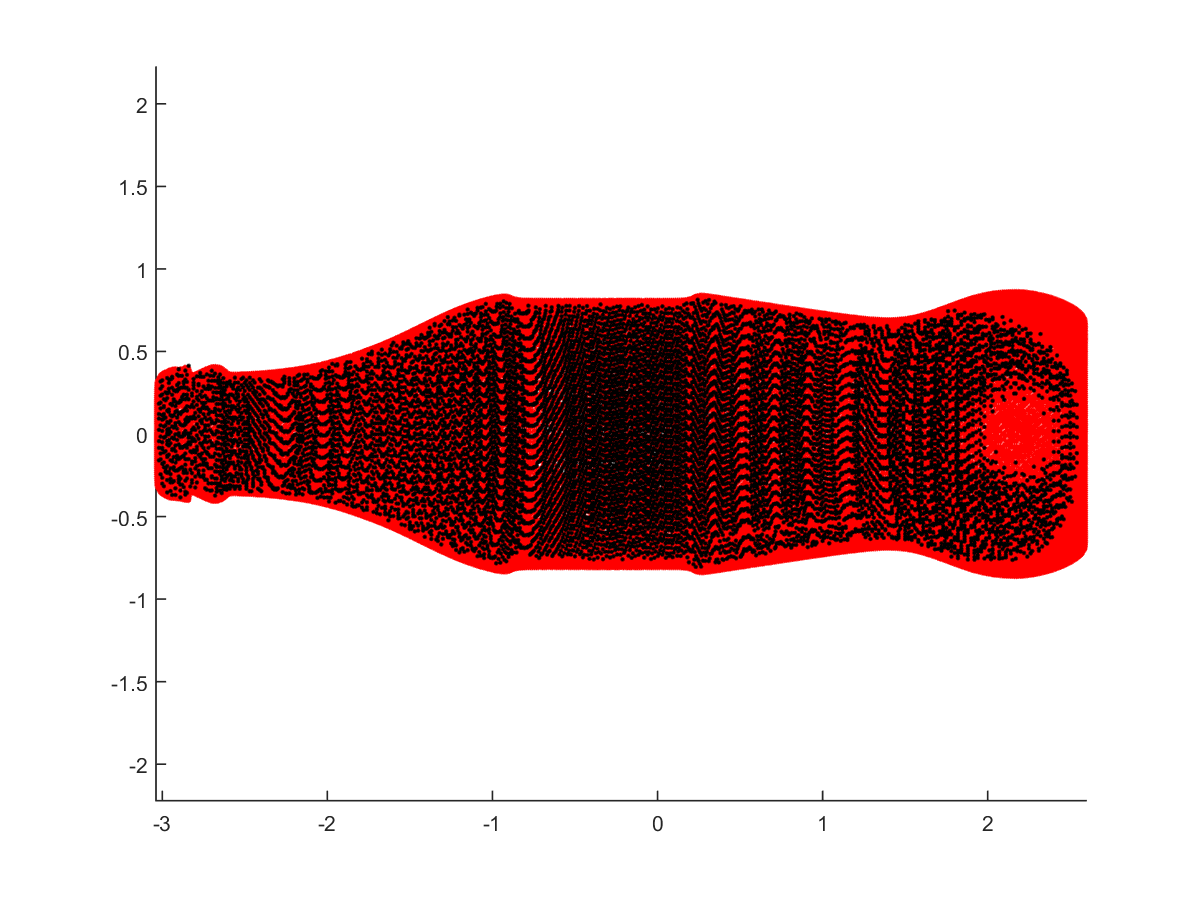
\includegraphics[width=0.2\textwidth]{interp/synth_data/bottle/bottle_sl_02080208.png}}\\
  & \multicolumn{4}{c}{(a). tex(0.2), alb(0.8), spec(0.2), rough(0.8)}\\
  EPS &
  \includegraphics[width=0.2\textwidth]{interp/synth_data/bottle/bottle_02080502}&
  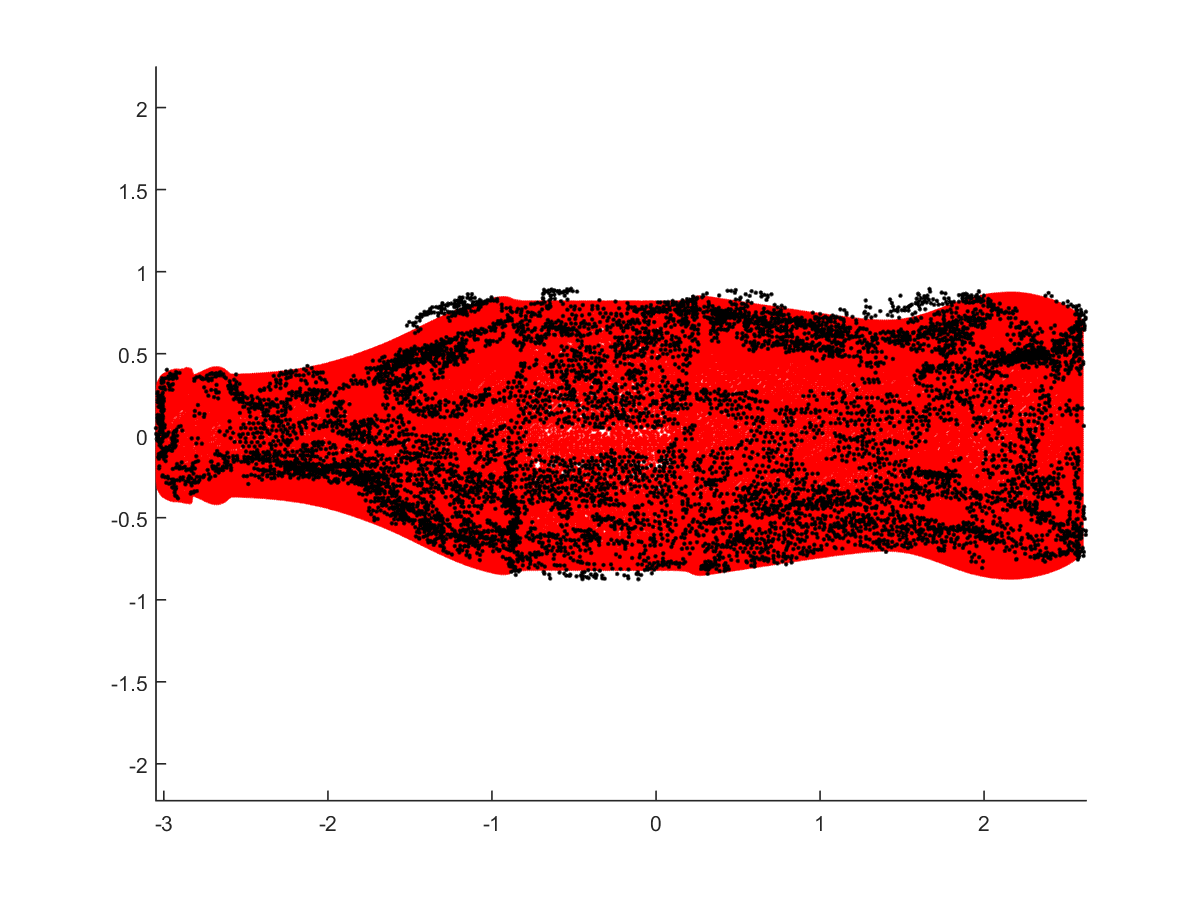
\includegraphics[width=0.2\textwidth]{interp/synth_data/bottle/bottle_mvs_02080502.png}&
  \fcolorbox{green}{white}{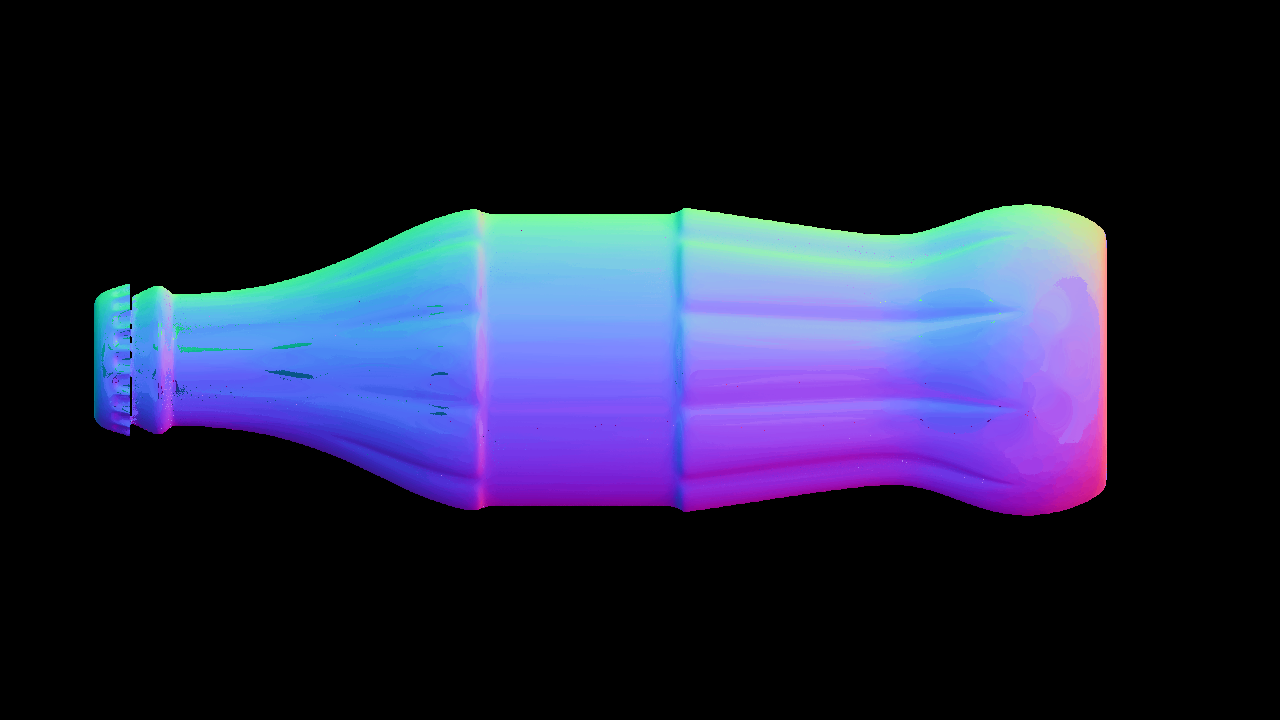
\includegraphics[width=0.2\textwidth]{interp/synth_data/bottle/bottle_ps_02080502.png}}&
  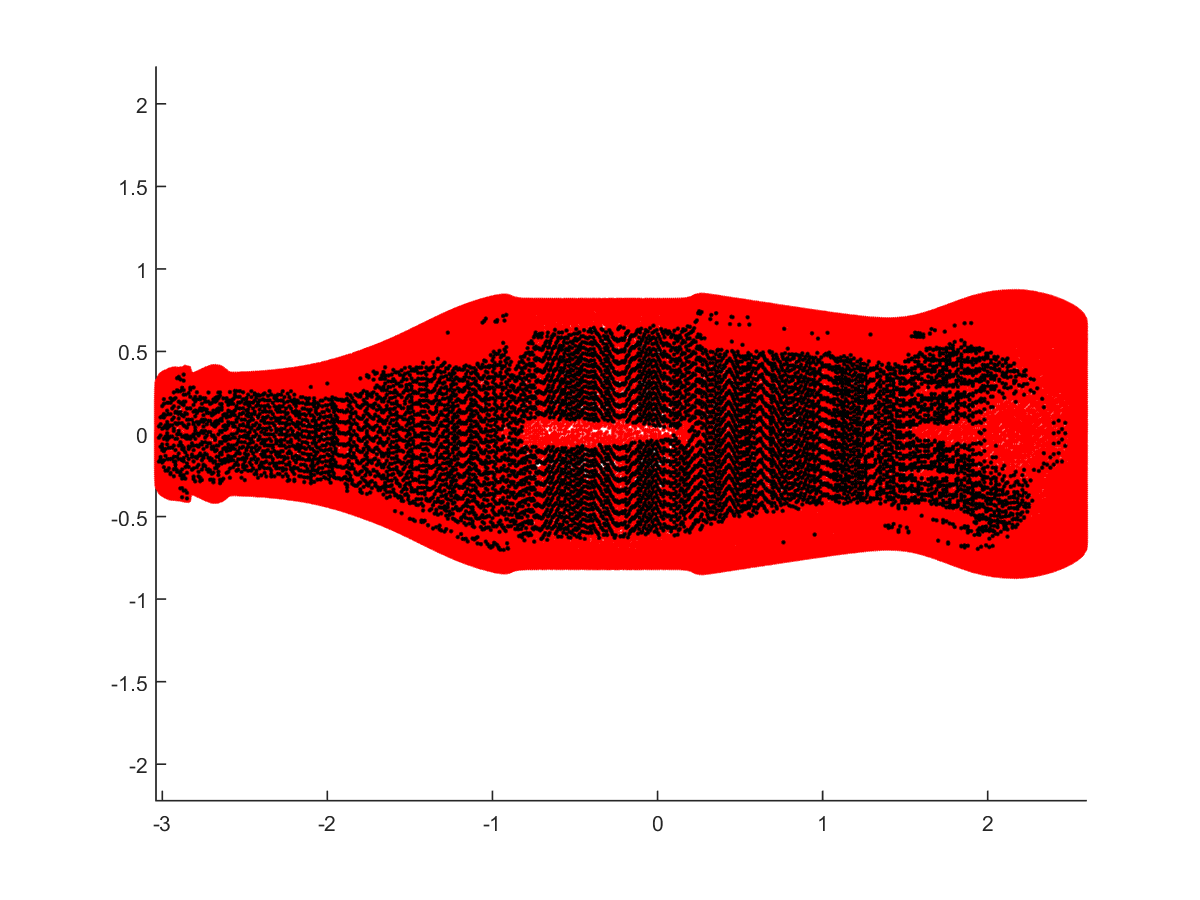
\includegraphics[width=0.2\textwidth]{interp/synth_data/bottle/bottle_sl_02080502.png}\\
  & \multicolumn{4}{c}{(b). tex(0.2), alb(0.8), spec(0.5), rough(0.2)}\\
  PMVS, EPS, GSL&
  \includegraphics[width=0.2\textwidth]{interp/synth_data/bottle/bottle_08080208}&
  \fcolorbox{green}{white}{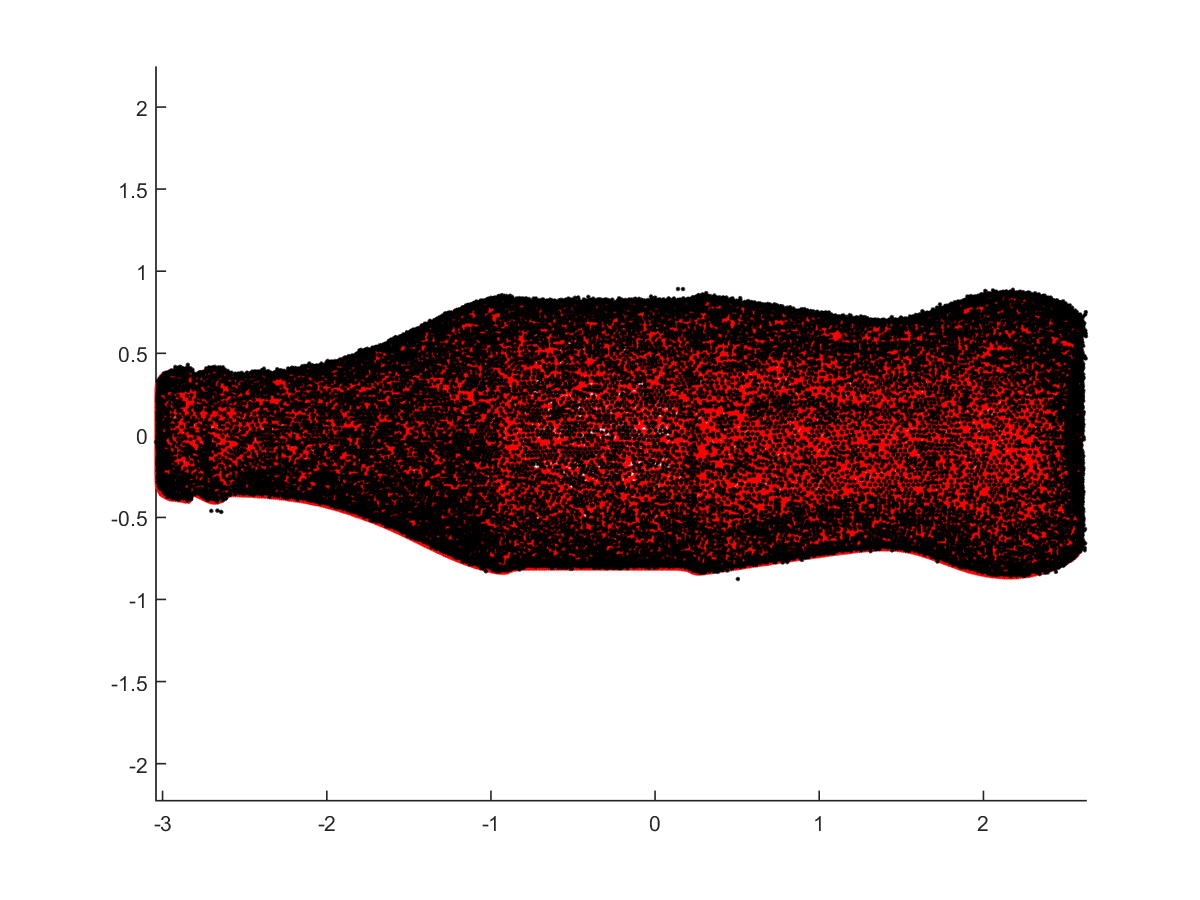
\includegraphics[width=0.2\textwidth]{interp/synth_data/bottle/bottle_mvs_08080208.png}}&
  \fcolorbox{green}{white}{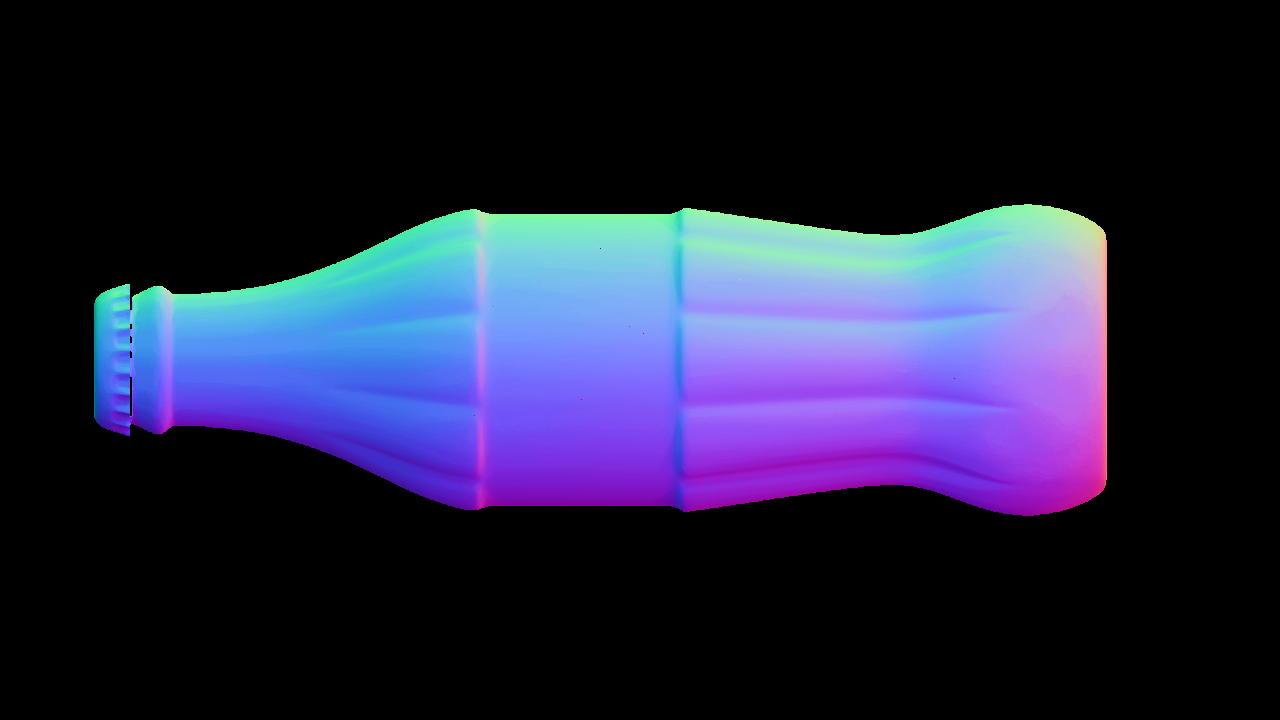
\includegraphics[width=0.2\textwidth]{interp/synth_data/bottle/bottle_ps_08080208.png}}&
  \fcolorbox{green}{white}{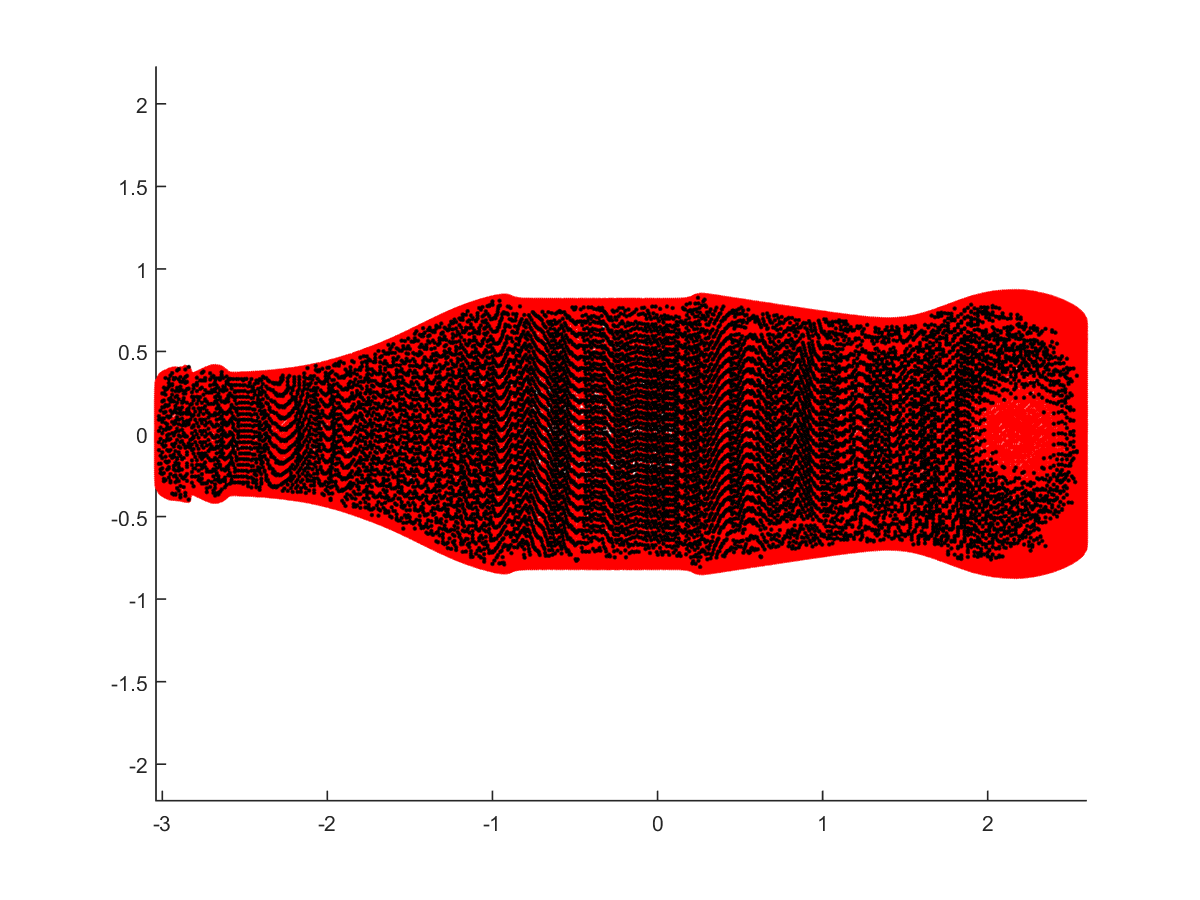
\includegraphics[width=0.2\textwidth]{interp/synth_data/bottle/bottle_sl_08080208.png}}\\
  & \multicolumn{4}{c}{(c). tex(0.8), alb(0.8), spec(0.2), rough(0.8)}\\
  PMVS, EPS&
  \includegraphics[width=0.2\textwidth]{interp/synth_data/bottle/bottle_08080502}&
  \fcolorbox{green}{white}{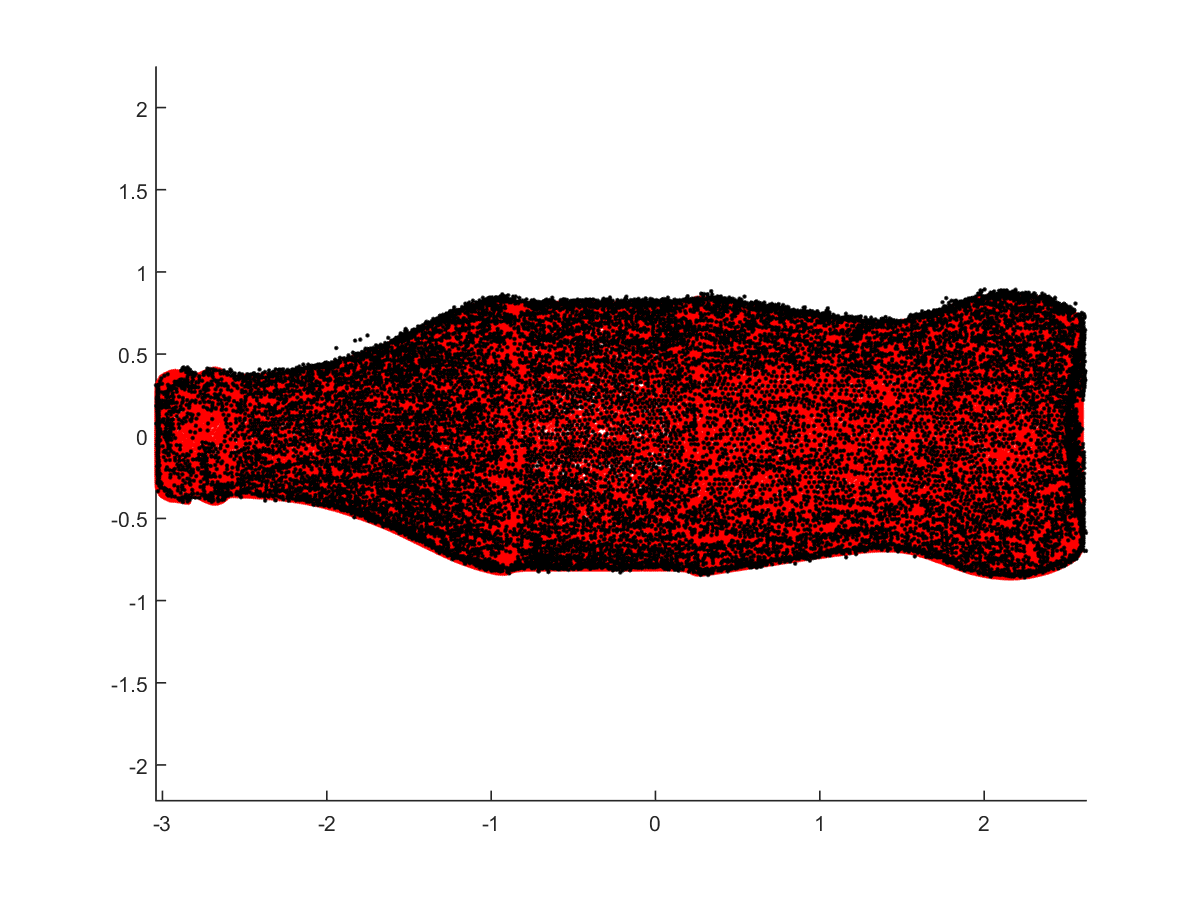
\includegraphics[width=0.2\textwidth]{interp/synth_data/bottle/bottle_mvs_08080502.png}}&
  \fcolorbox{green}{white}{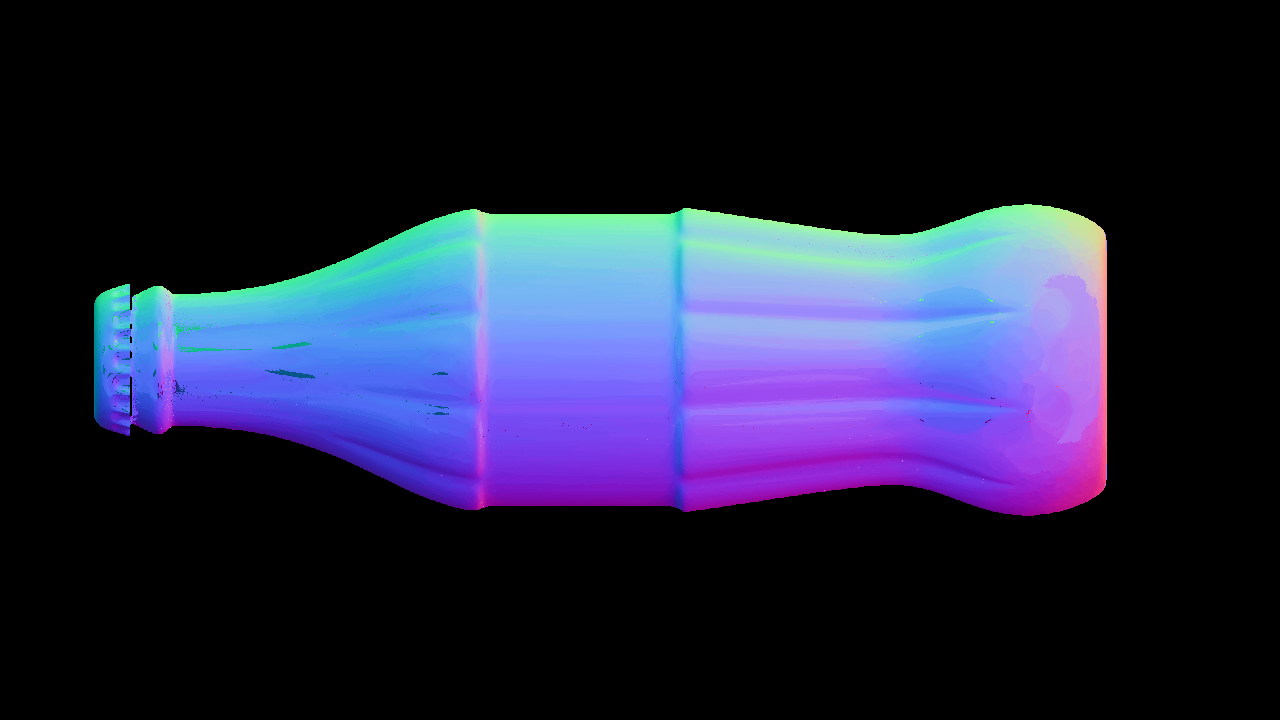
\includegraphics[width=0.2\textwidth]{interp/synth_data/bottle/bottle_ps_08080502.png}}&
  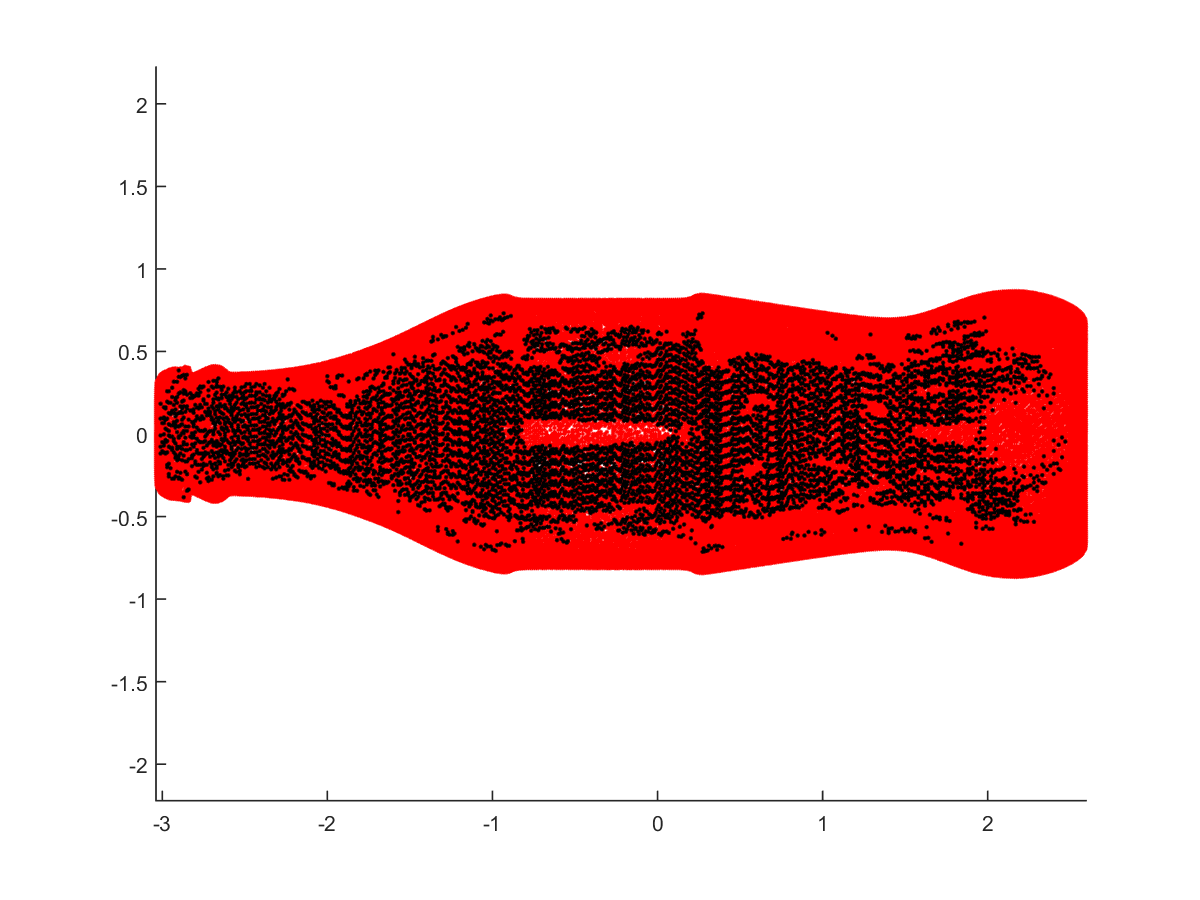
\includegraphics[width=0.2\textwidth]{interp/synth_data/bottle/bottle_sl_08080502.png}\\
  & \multicolumn{4}{c}{(d). tex(0.8), alb(0.8), spec(0.5), rough(0.2)}\\
  \hline
  ~ & ~ & MVS & PS & SL\\
\end{tabular}
\caption{The first column shows the best algorithm chosen by the mapping. The quantitative and qualitative performance of each technique on the synthetic dataset is also shown. The red dots represent the ground truth while the black dots represent the reconstruction.}
\label{fig:synth_data_results_bottle}
\end{sidewaysfigure}

\subsubsection{Data 2: knight}
The second object is a knight chess piece, which has medium concavity. In this case, we can see that the results of PMVS and GSL are still consistent with the mapping. However, the EPS fails to return reliable reconstruction in cases of high specular, such as (b) and (d), which is manifested by an increase in the variation of the angular error, represented by standard variation and the interquartile range. Thus, we claim that the mapping is still valid for PMVS, GSL and for EPS in low specular cases.
\begin{sidewaysfigure}[!htbp]
\centering
\begin{tabular}{c|ccccc}
  Mapping & Quantitative results & ~ & Qualitative results & ~\\
  \hline
  EPS, GSL & 
  \includegraphics[width=0.2\textwidth]{interp/synth_data/knight/knight_02080208}&
  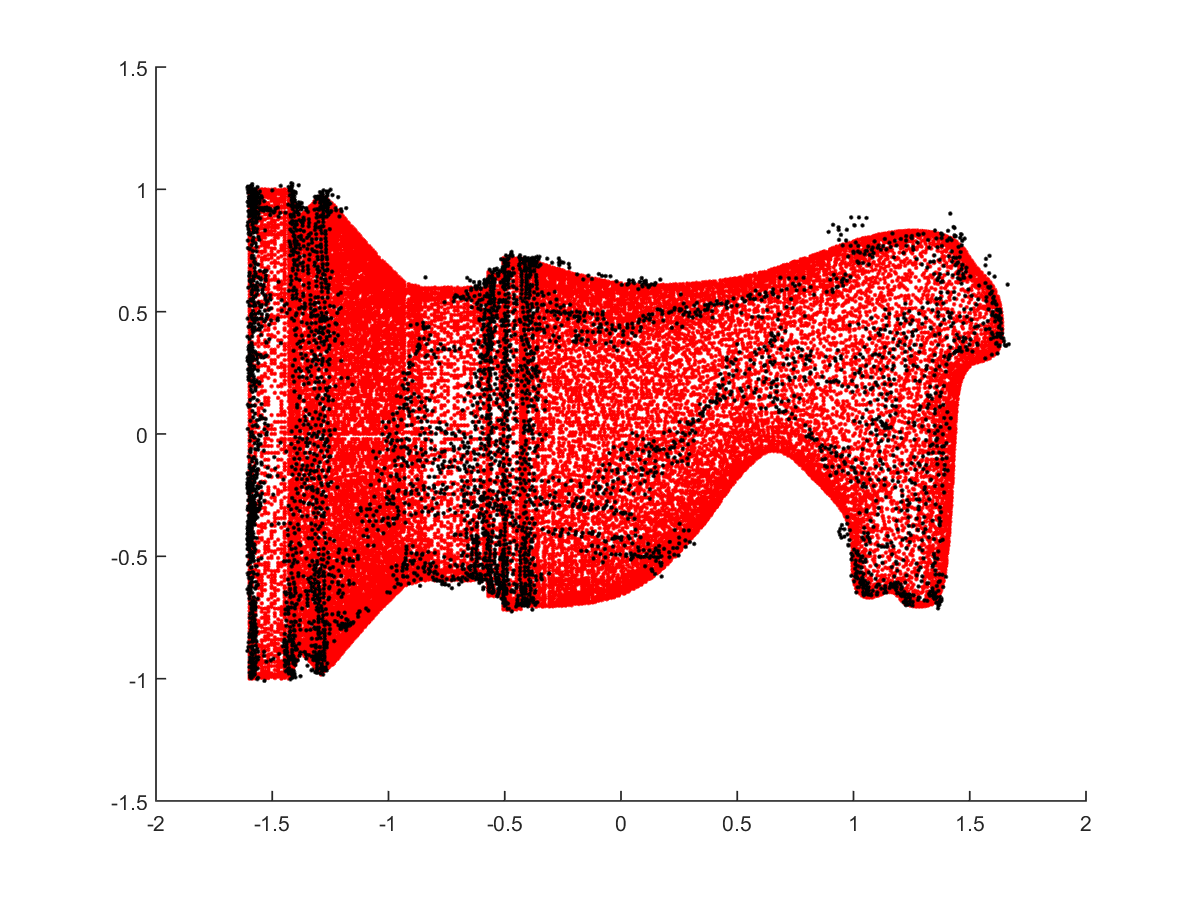
\includegraphics[width=0.2\textwidth]{interp/synth_data/knight/knight_mvs_02080208.png}&
  \fcolorbox{green}{white}{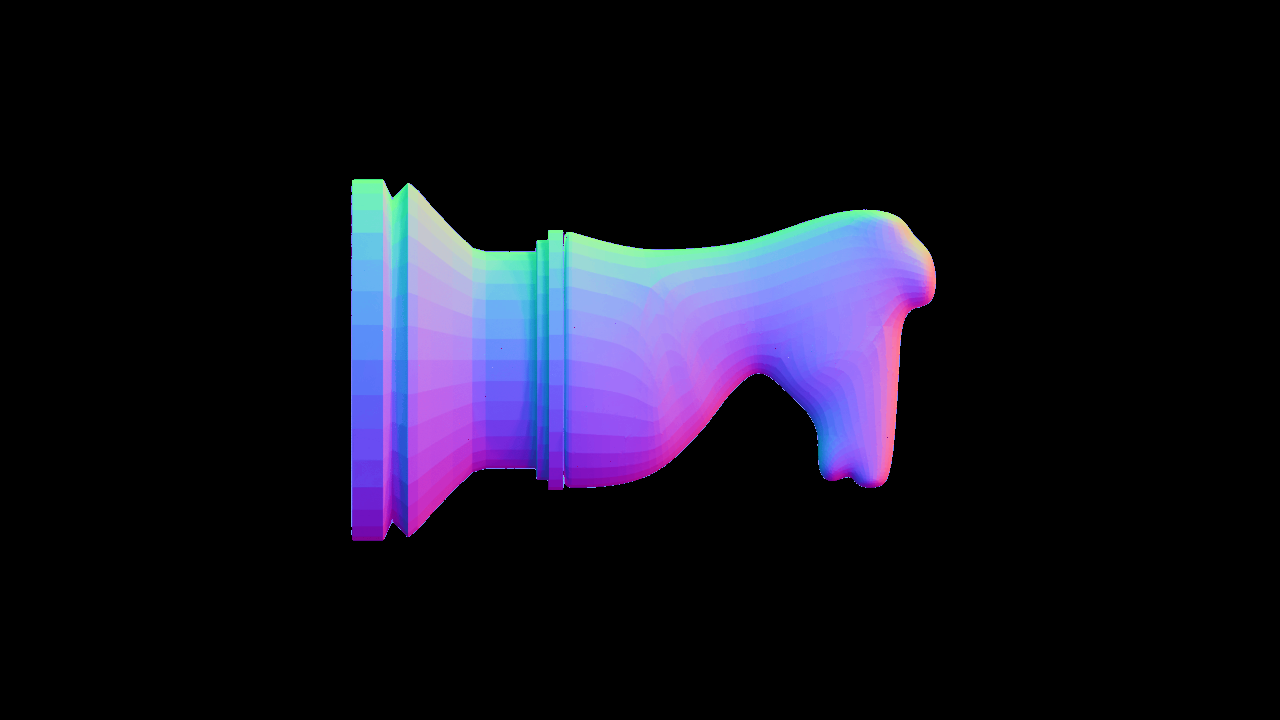
\includegraphics[width=0.2\textwidth]{interp/synth_data/knight/knight_ps_02080208.png}}&
  \fcolorbox{green}{white}{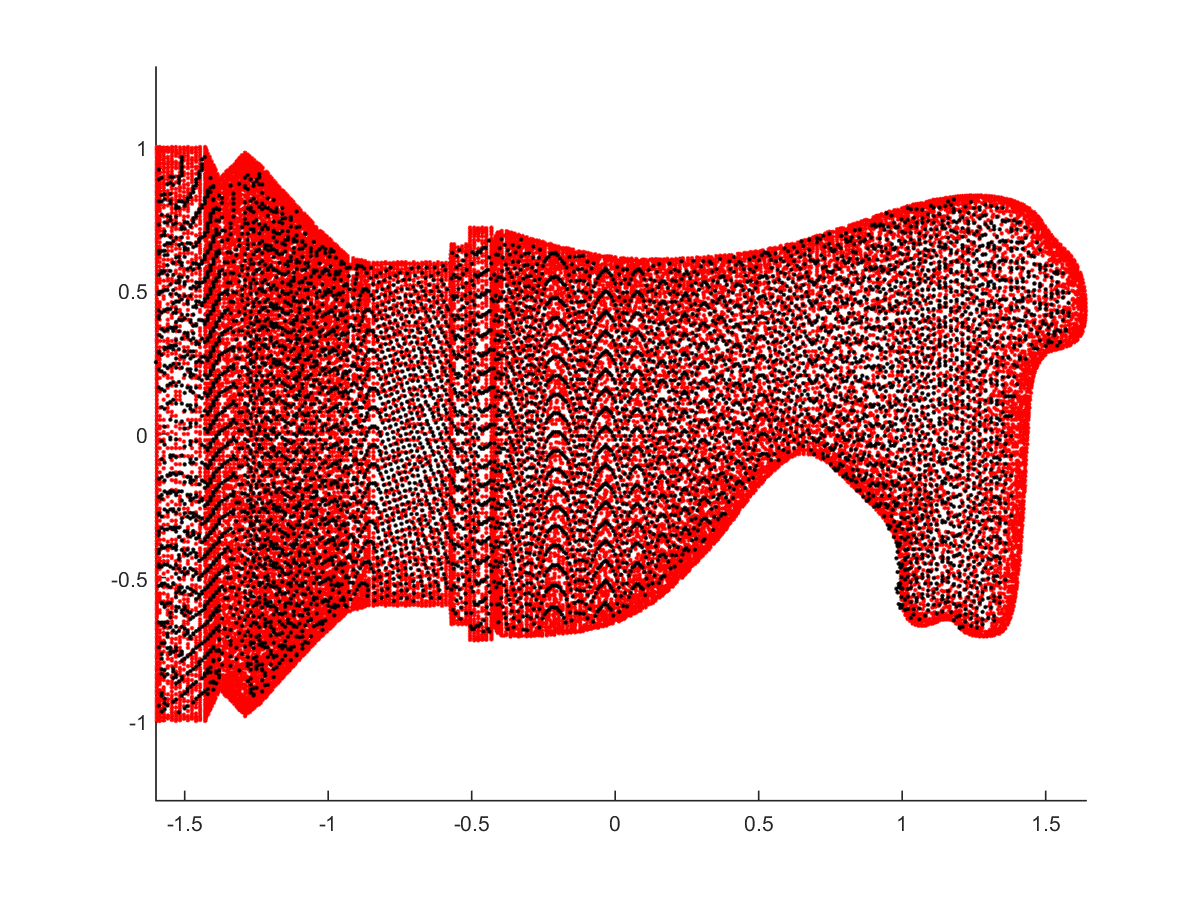
\includegraphics[width=0.2\textwidth]{interp/synth_data/knight/knight_sl_02080208.png}}\\
  & \multicolumn{4}{c}{(a). tex(0.2), alb(0.8), spec(0.2), rough(0.8)}\\
  EPS &
  \includegraphics[width=0.2\textwidth]{interp/synth_data/knight/knight_02080502}&
  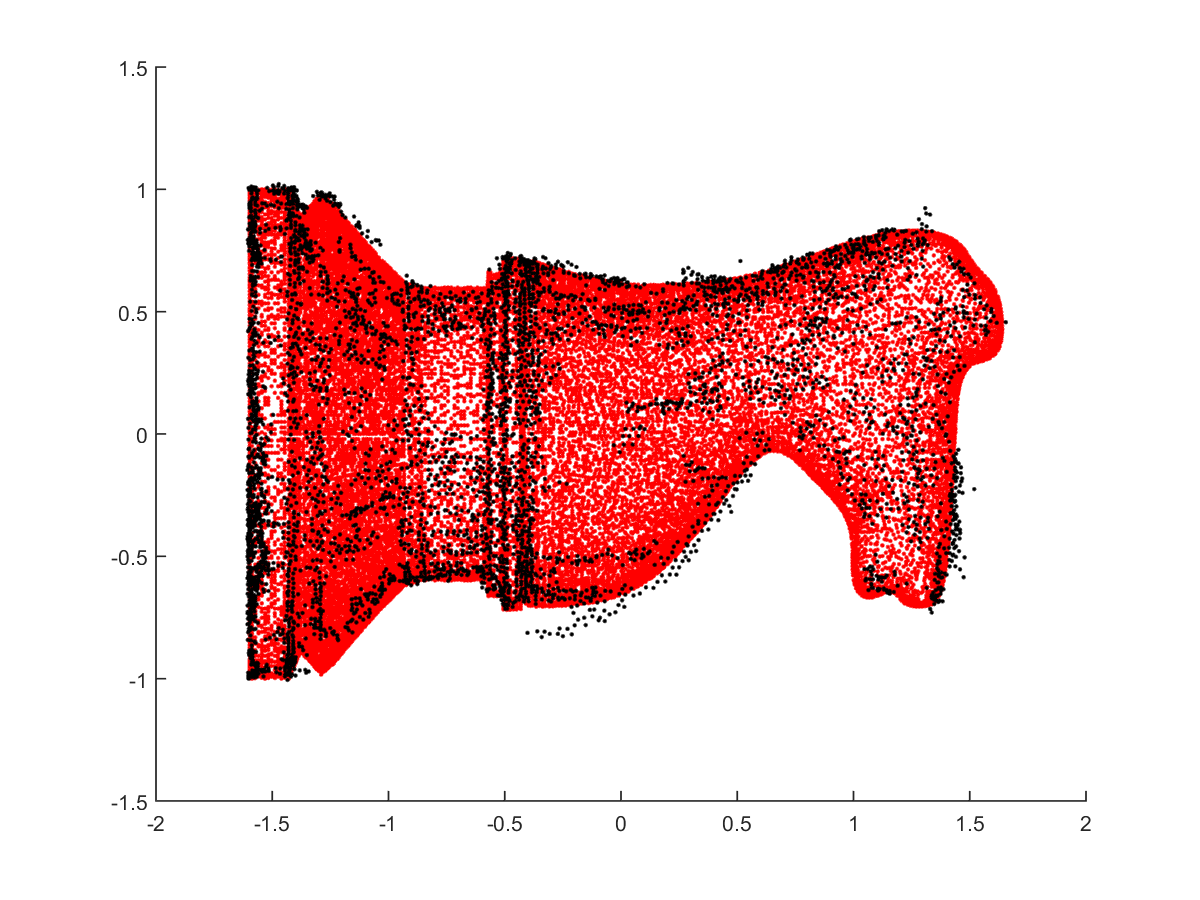
\includegraphics[width=0.2\textwidth]{interp/synth_data/knight/knight_mvs_02080502.png}&
  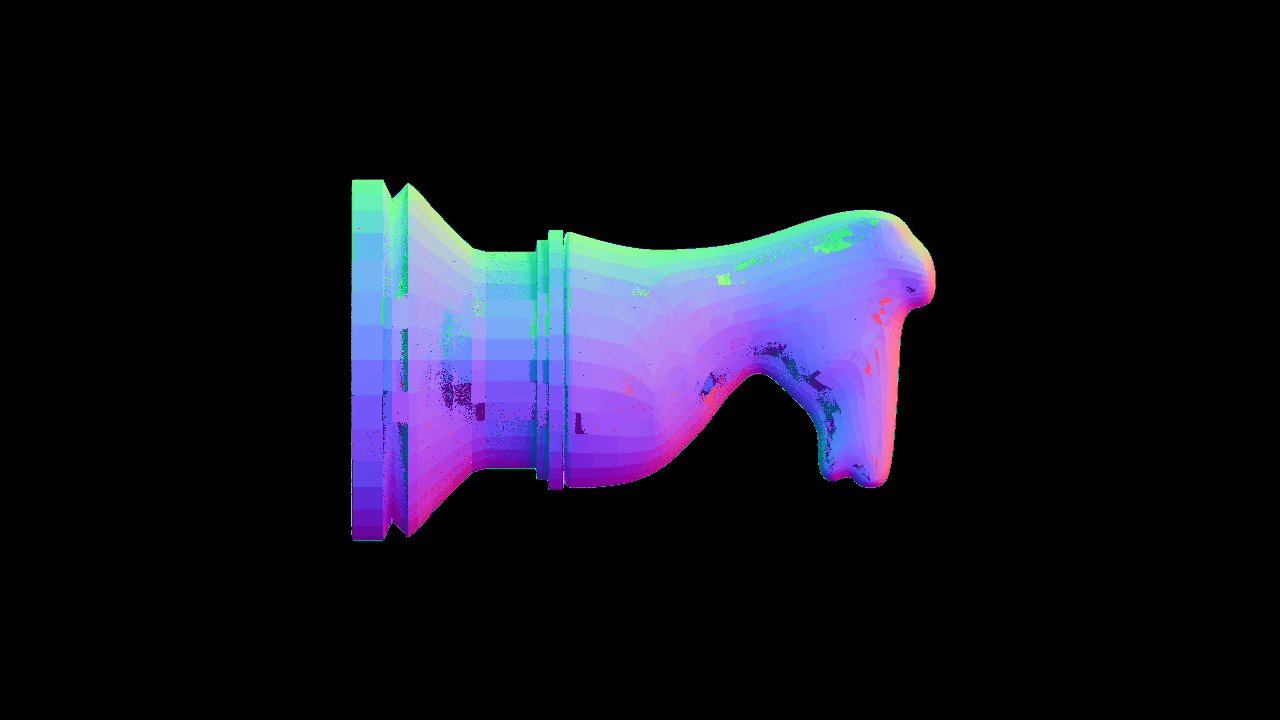
\includegraphics[width=0.2\textwidth]{interp/synth_data/knight/knight_ps_02080502.png}&
  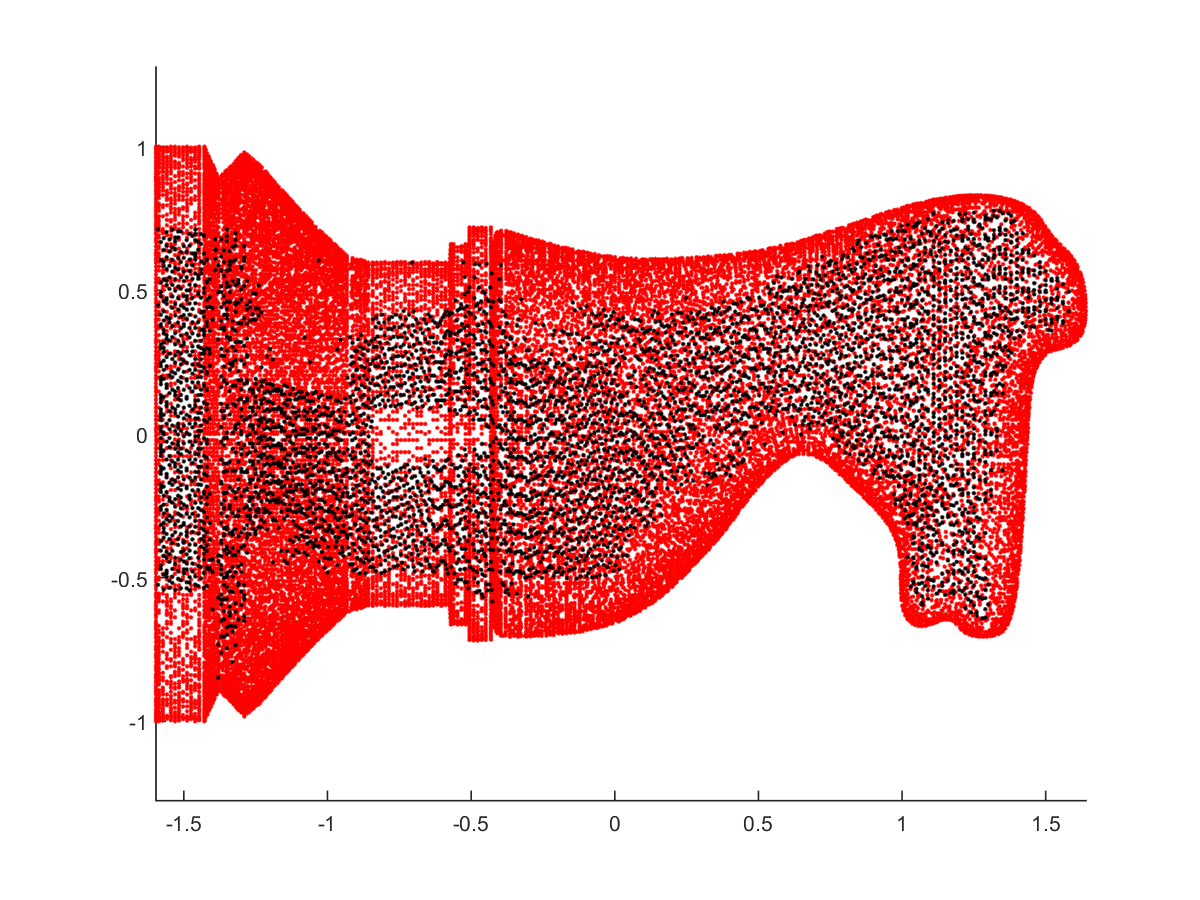
\includegraphics[width=0.2\textwidth]{interp/synth_data/knight/knight_sl_02080502.png}\\
  & \multicolumn{4}{c}{(b). tex(0.2), alb(0.8), spec(0.5), rough(0.2)}\\
  PMVS, EPS, GSL&
  \includegraphics[width=0.2\textwidth]{interp/synth_data/knight/knight_08080208}&
  \fcolorbox{green}{white}{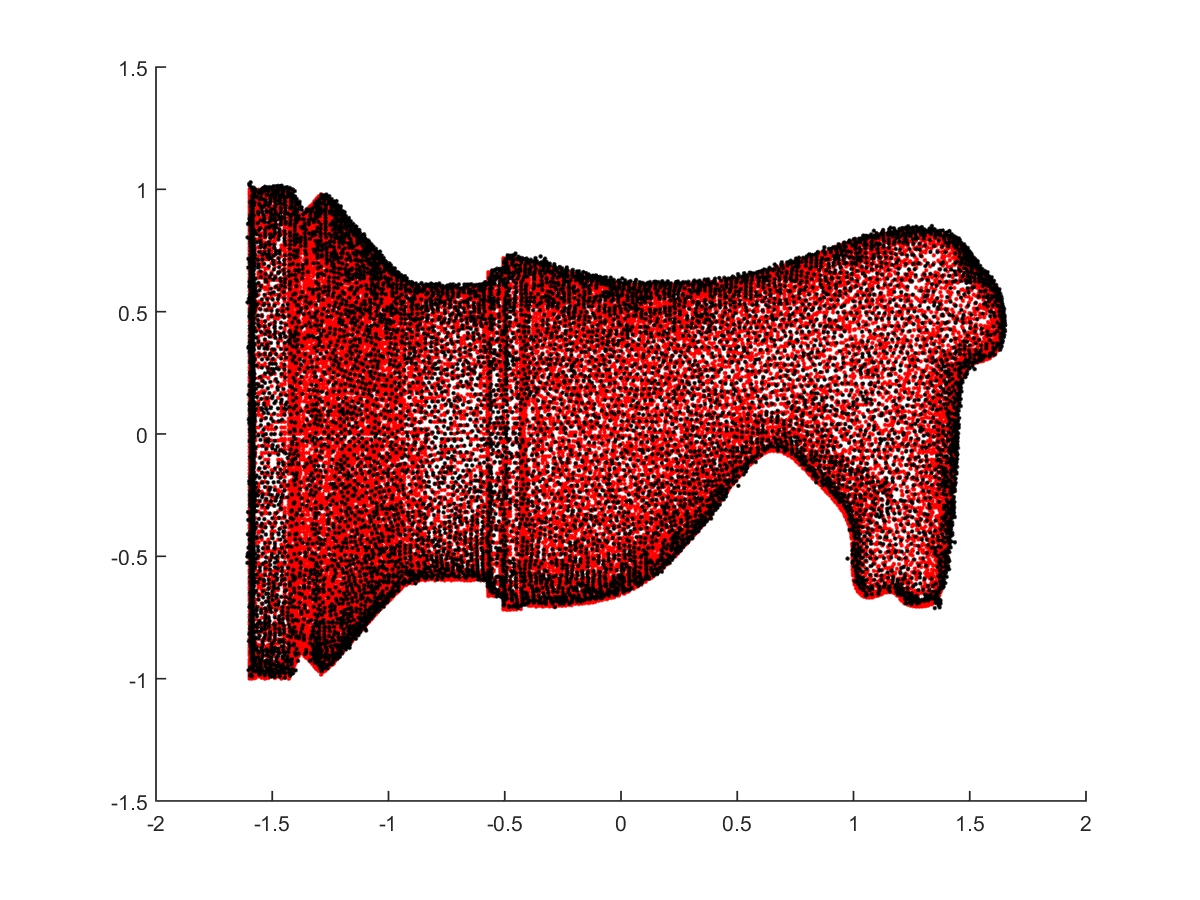
\includegraphics[width=0.2\textwidth]{interp/synth_data/knight/knight_mvs_08080208.png}}&
  \fcolorbox{green}{white}{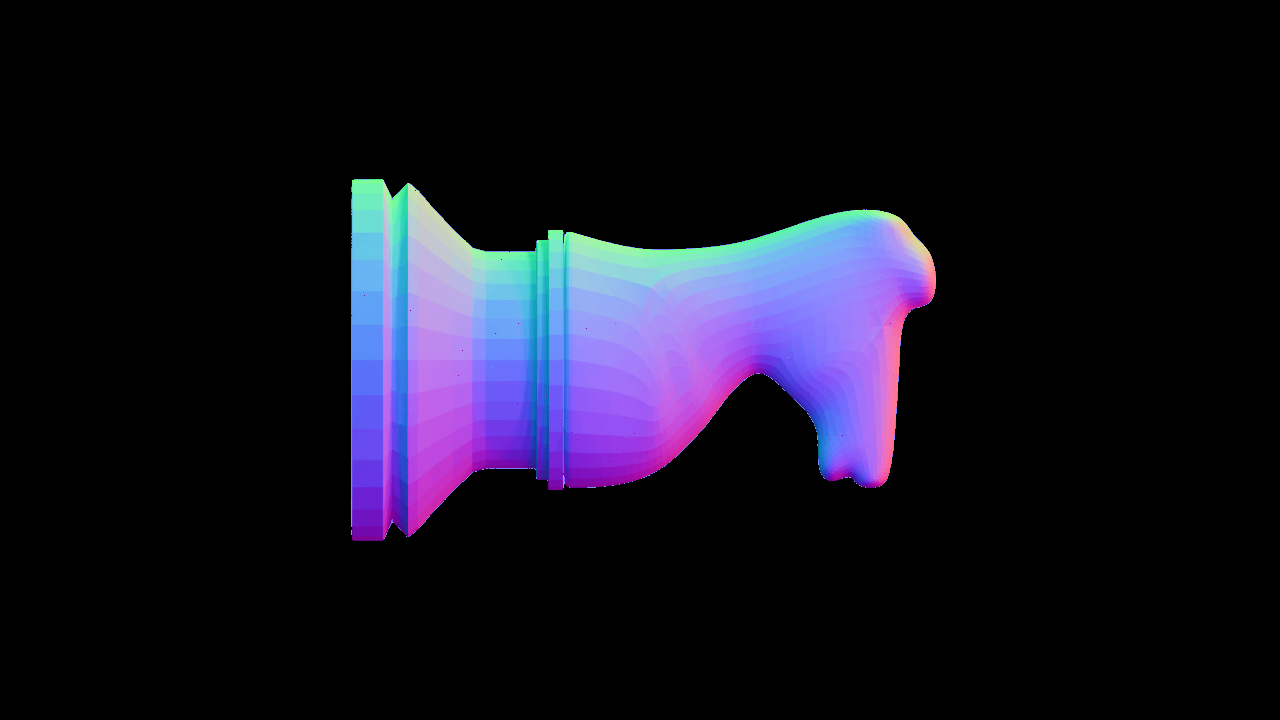
\includegraphics[width=0.2\textwidth]{interp/synth_data/knight/knight_ps_08080208.png}}&
  \fcolorbox{green}{white}{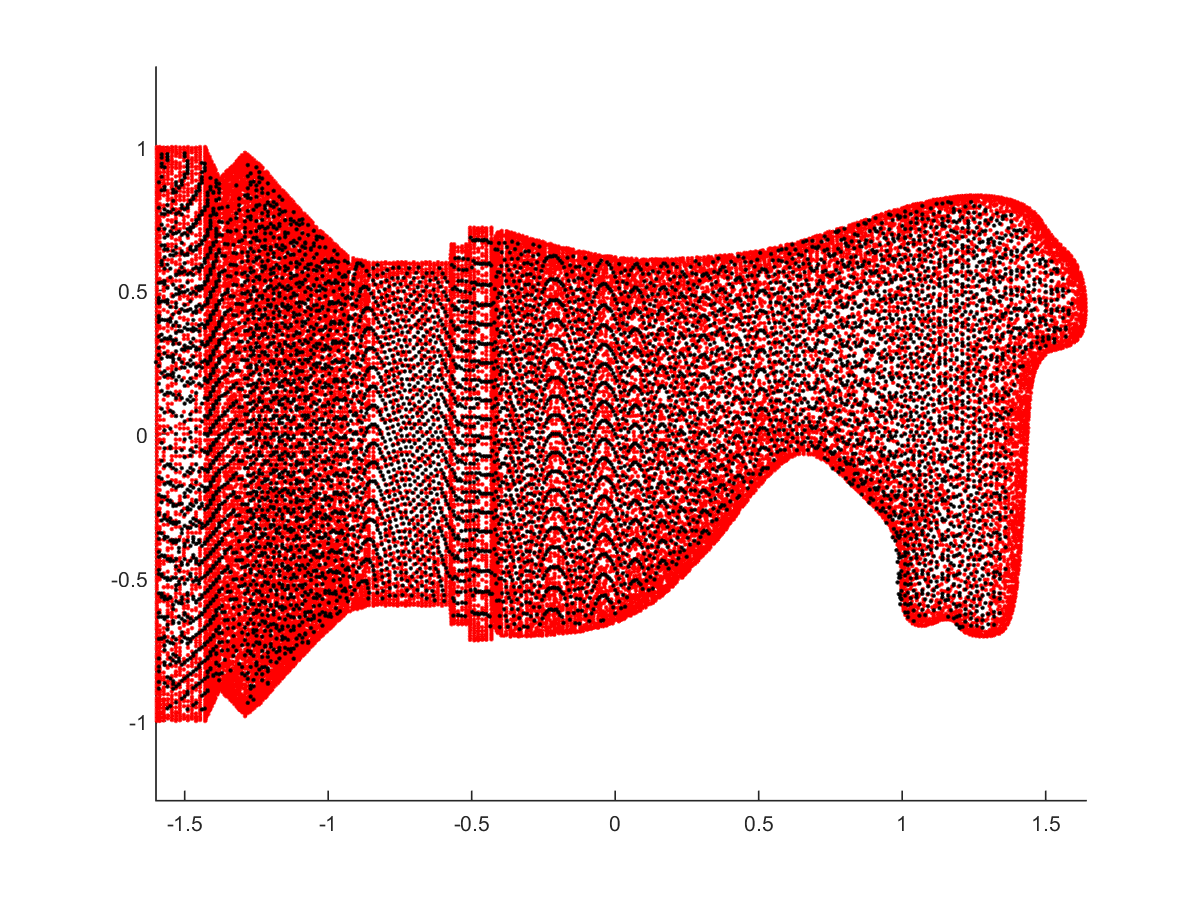
\includegraphics[width=0.2\textwidth]{interp/synth_data/knight/knight_sl_08080208.png}}\\
  & \multicolumn{4}{c}{(c). tex(0.8), alb(0.8), spec(0.2), rough(0.8)}\\
  PMVS, EPS&
  \includegraphics[width=0.2\textwidth]{interp/synth_data/knight/knight_08080502}&
  \fcolorbox{green}{white}{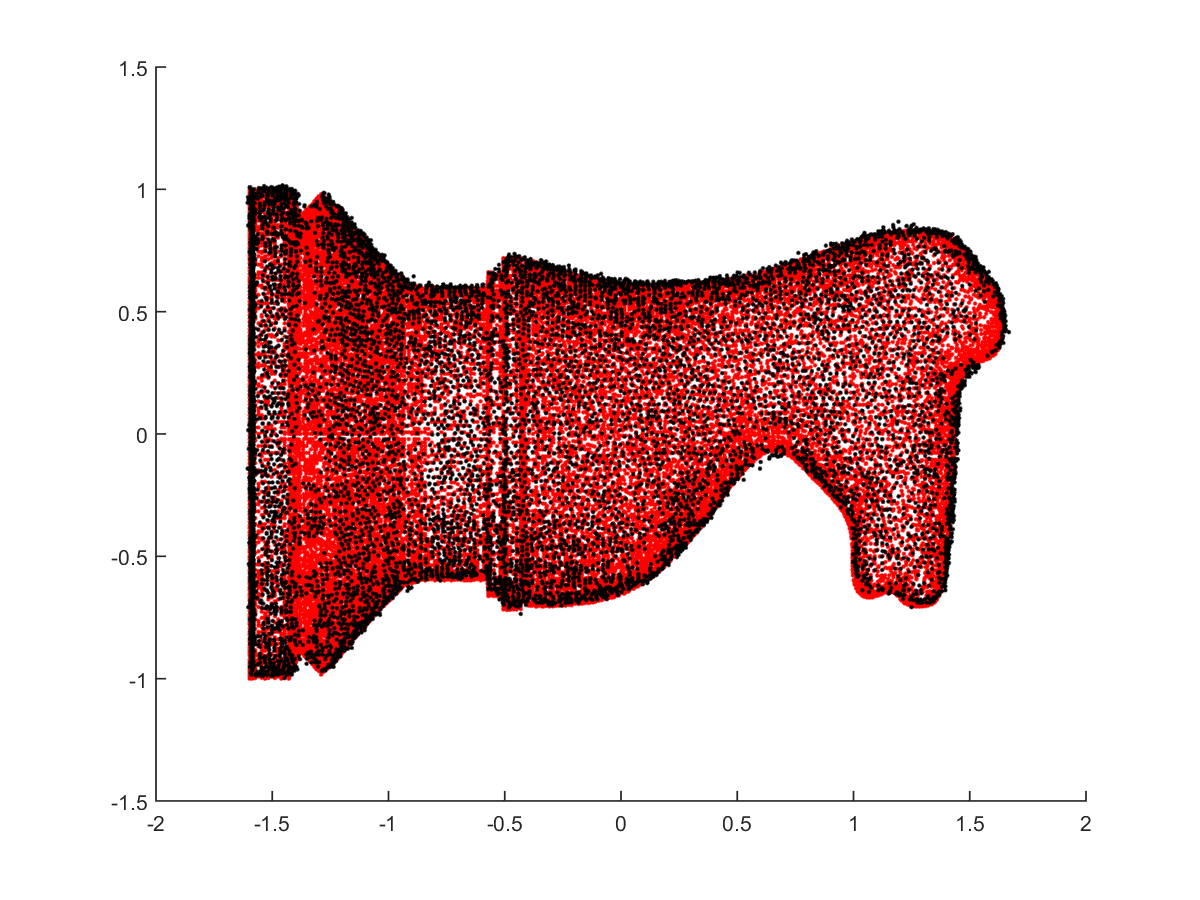
\includegraphics[width=0.2\textwidth]{interp/synth_data/knight/knight_mvs_08080502.png}}&
  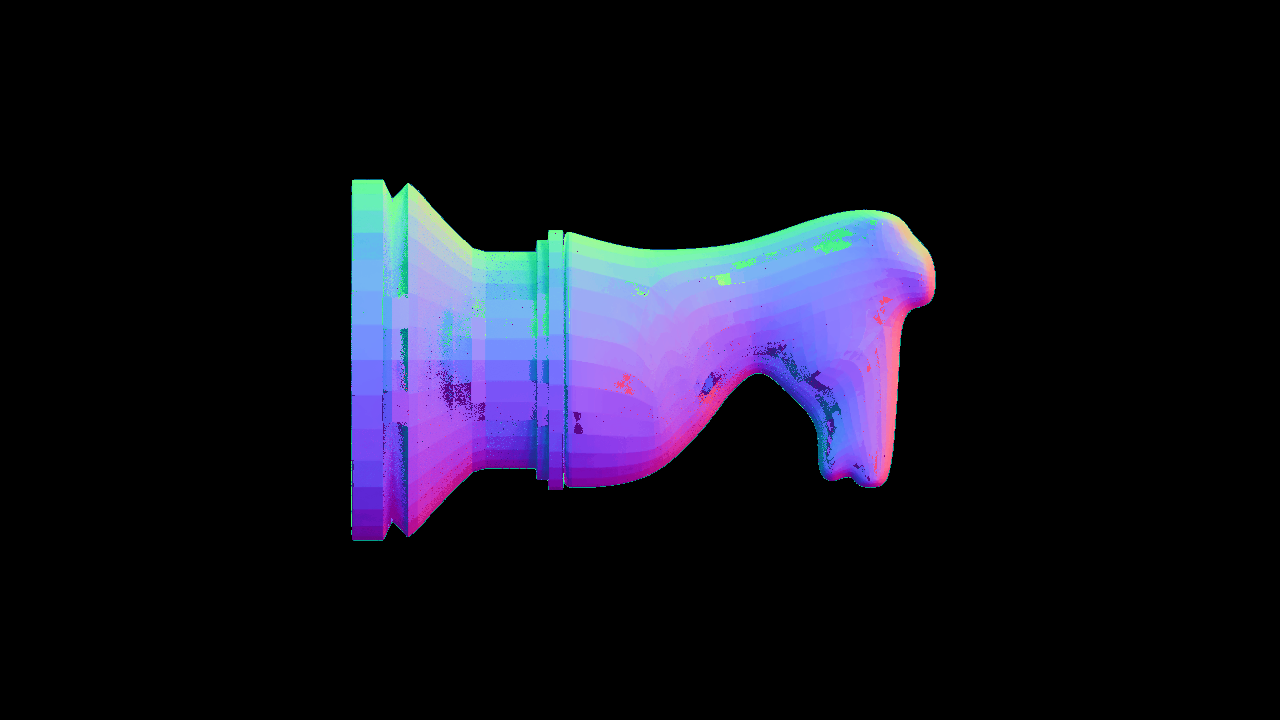
\includegraphics[width=0.2\textwidth]{interp/synth_data/knight/knight_ps_08080502.png}&
  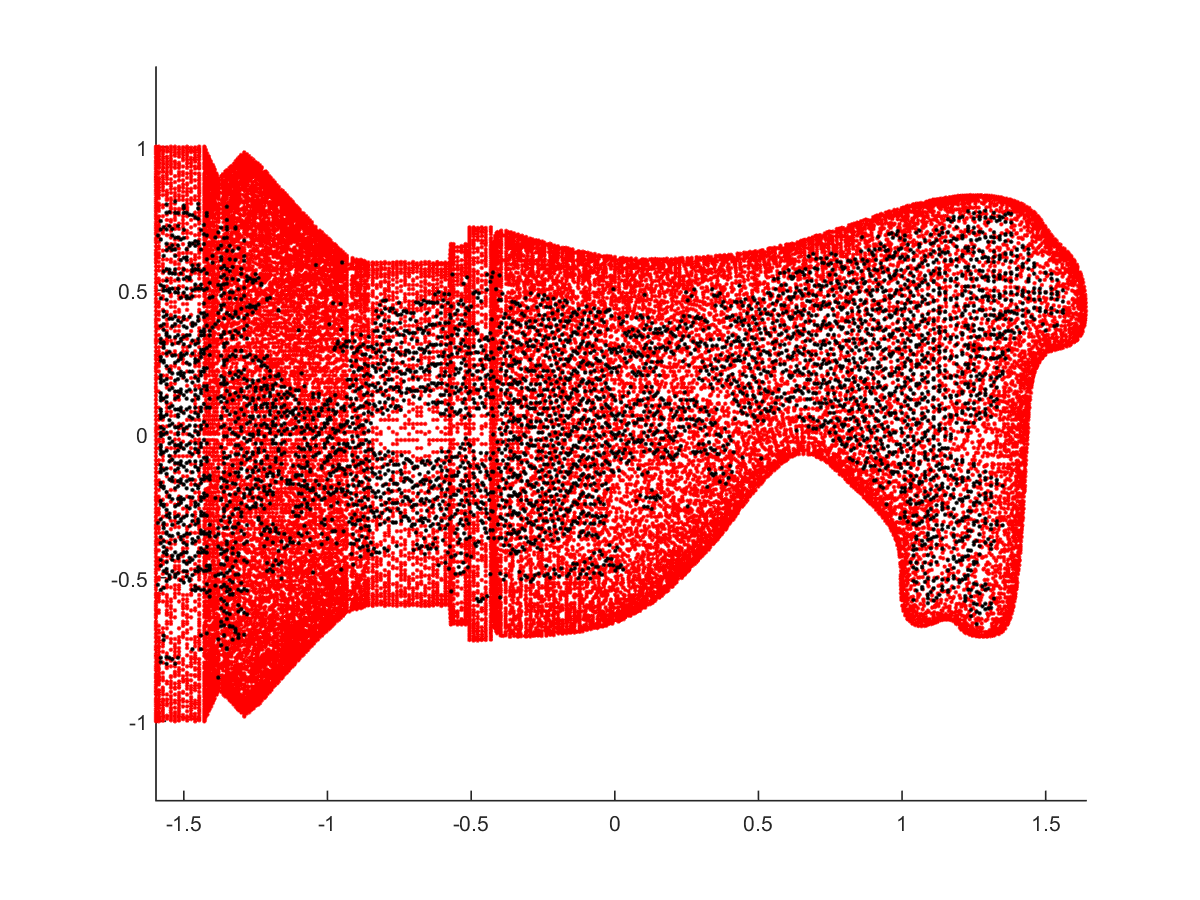
\includegraphics[width=0.2\textwidth]{interp/synth_data/knight/knight_sl_08080502.png}\\
  & \multicolumn{4}{c}{(d). tex(0.8), alb(0.8), spec(0.5), rough(0.2)}\\
  \hline
  ~ & ~ & MVS & PS & SL\\
\end{tabular}
\caption{The first column shows the best algorithm chosen by the mapping. The quantitative and qualitative performance of each technique on the synthetic dataset is also shown. The red dots represent the ground truth while the black dot represent the reconstruction.}
\label{fig:synth_data_results_knight}
\end{sidewaysfigure}

\subsubsection{Data 3: king}
The last synthetic object is the king chess piece, which has the largest concavity. In the case of high concavity, quantitative results of PMVS and GSL are still consistent with that of the mapping. However, the results of the EPS become inconsistent, which is a result of the cast shadow from the large concavity. Though the result of EPS under conditions (a) and (c) are still better than that of the baseline, the median angular error is above the acceptable threshold, which is $10^\circ$ in most cases. We can see with more clarity from the normal maps that the cast shadow on the `cross' leads to completely inaccurate normal estimation, which is labeled by a red rectangle.
\begin{sidewaysfigure}[!htbp]
\centering
\begin{tabular}{c|ccccc}
  Mapping & Quantitative results & ~ & Qualitative results & ~\\
  \hline
  EPS, GSL & 
  \includegraphics[width=0.2\textwidth]{interp/synth_data/king/king_02080208}&
  \includegraphics[width=0.2\textwidth]{interp/synth_data/king/king_mvs_02080208.png}&
  \includegraphics[width=0.2\textwidth]{interp/synth_data/king/king_ps_02080208.png}&
  \fcolorbox{green}{white}{\includegraphics[width=0.2\textwidth]{interp/synth_data/king/king_sl_02080208.png}}\\
  & \multicolumn{4}{c}{(a). tex(0.2), alb(0.8), spec(0.2), rough(0.8)}\\
  EPS &
  \includegraphics[width=0.2\textwidth]{interp/synth_data/king/king_02080502}&
  \includegraphics[width=0.2\textwidth]{interp/synth_data/king/king_mvs_02080502.png}&
  \includegraphics[width=0.2\textwidth]{interp/synth_data/king/king_ps_02080502.png}&
  \includegraphics[width=0.2\textwidth]{interp/synth_data/king/king_sl_02080502.png}\\
  & \multicolumn{4}{c}{(b). tex(0.2), alb(0.8), spec(0.5), rough(0.2)}\\
  PMVS, GSL, EPS&
  \includegraphics[width=0.2\textwidth]{interp/synth_data/king/king_08080208}&
  \fcolorbox{green}{white}{\includegraphics[width=0.2\textwidth]{interp/synth_data/king/king_mvs_08080208.png}}&
  \includegraphics[width=0.2\textwidth]{interp/synth_data/king/king_ps_08080208.png}&
  \fcolorbox{green}{white}{\includegraphics[width=0.2\textwidth]{interp/synth_data/king/king_sl_08080208.png}}\\
  & \multicolumn{4}{c}{(c). tex(0.8), alb(0.8), spec(0.2), rough(0.8)}\\
  PMVS, EPS&
  \includegraphics[width=0.2\textwidth]{interp/synth_data/king/king_08080502}&
  \fcolorbox{green}{white}{\includegraphics[width=0.2\textwidth]{interp/synth_data/king/king_mvs_08080502.png}}&
  \includegraphics[width=0.2\textwidth]{interp/synth_data/king/king_ps_08080502.png}&
  \includegraphics[width=0.2\textwidth]{interp/synth_data/king/king_sl_08080502.png}\\
  & \multicolumn{4}{c}{(d). tex(0.8), alb(0.8), spec(0.5), rough(0.2)}\\
  \hline
  ~ & ~ & MVS & PS & SL\\
\end{tabular}
\caption{The first column shows the best algorithm chosen by the mapping. The quantitative and qualitative performance of each technique on the synthetic dataset is also shown. The green dots represent the ground truth while the black dots represent the reconstruction.}
\label{fig:synth_data_results_king}
\end{sidewaysfigure}

\subsubsection{Summary}
We can conclude that the mapping of PMVS and GSL are robust to concavity, whereas EPS is relatively more sensitive to concavity due to cast shadows. Therefore, we should redirect more research efforts to developing Photometric Stereo algorithms that can reliably deal with cast shadow so that they can be reliably applied to more complex shapes.
% \textbf{(a), (b)} In Figure~\ref{fig:synth_data_results} (a), the mapping predicts that EPS and GSL can give satisfactory results, which is consistent to the quantitative result shown in column 2 and the qualitative resulted labeled in green rectangle. The completeness of the PMVS is low due to the lack of texture.

% \textbf{(c), (d)} In Figure~\ref{fig:synth_data_results} (a), the mapping predicts that all three methods can give satisfactory results, which is consistent to the quantitative result shown in column 2 and the qualitative resulted labeled in green rectangle.

\section{Interpreter}
\label{sec:interp}
Our framework consists of three separate layers. The upper layer is the description of the problem domain. The middle layer is the interpreter which receives a description from the user and return an acceptable result. The bottom layer is the actual implementation of the algorithms. The interpreter is responsible for choosing an appropriate 3D reconstruction algorithm based on the description of the problem domain and additional requirements. Thus, it requires an understanding of algorithmic performance across difference ranges of problem space to create a suitable interpreter. There are many ways to use the mapping to interpret the problem description. We proposed a proof of concetp interpreter that consists of two components: mapping and constraints.
\begin{figure}[!htbp]
\centering
\begin{tikzpicture}[node distance=1.2cm, auto]

\node (mapping) [data_nonfixed] {Mapping};
\node (constraint) [data_nonfixed, right of=mapping, xshift=1cm] {Constraints};
\draw[red,thick,solid] ($(mapping.north west)+(-0.3,0.3)$)  rectangle ($(constraint.south east)+(0.3,-0.3)$);

\end{tikzpicture}
\caption{Two components of the Interpreter layer.}
\label{fig:interpreter_layer}
\end{figure}

The mapping constructed using the synthetic dataset from Chapter~\ref{ch:3DRecon_Mapping} provides us with a detailed understanding of how different combinations of properties affect the performance of algorithms. This allows us to select an appropriate algorithm based on a description of properties.
% When multiple algorithms are appropriate, we use a very simple ranking system based on the metrics: if one algorithm has the same completeness but is more accurate, or more complete and equally accurate, it is chosen over the others. (This ranking also allows us to define an efficiency versus accuracy tradeoff for the developer to use.) We could also choose to execute more than one algorithm and accept the results of the one which performed best - however measuring this may be challenging.

Next we turn to defining the constraints of the framework. Constraints are provided to allow the user to describe the expected result so that a model best resembling the user's request can be returned by the framework when multiple algorithms achieve satisfactory results. The following constraints are provided: 
\begin{itemize}
\item Depth-first/shape-first: methods that reconstructs surface orientations from a single viewpoint cannot retrieve the depth information, and thus are refered to as 2.5D reconstruction. Examples of this are Shape from Shading, Photometric Stereo, and Shape from (de)focus, \etc. However, these methods generally can reconstruct fine scale details, thus can achieve results with much higher quality. Intuitively, depth-first can return model with true depth information whereas shape-first prioritizes fine details over depth information.
\item Accuracy-first/completeness-first: methods that achieve high accuracy do not necessary achieve high completeness. In light of this, the user can choose an algorithm based on the priority level of accuracy and completeness.
\end{itemize}

Under our current interpreter, if a developer-defiend description and constraints have more than one corresponding algorithm available, by default, depth-first has higher priority over quality-first, and accuracy has higher priority over completeness. Since GSL typically generates more accurate resutlts, the order of the algorithms is: GSL $>$ PMVS $>$ EPS.

\section{Evaluation of Interpreter}
\label{sec:eval_interp}
We demonstrate real-world use cases of the proof of concept interpreter, which should return a satisfactory result given a valid description, or a less successful one given an incorrect description. We choose four different problem conditions where each desrcibes one of the four major classes of objects and provides demonstrative results. Please refer to the appendix for more results.

\subsection{Synthetic Datasets}
We generate a dataset of four objects, each representing one of the four classes discussed in Section~\ref{ch:3DRecon_Taxo}. The mapping from problem conditions to algorithms are summarized in Table~\ref{tab:synth_prop_list}. Given a specific algorihthm, the proof-of-concept interpreter will select an algorithm, and any object that matches this description should be well reconstructed by this algorithm. We use four descriptions that match the four problem conditions listed in Table so that each object should at least return one well reconstructed result. Since a problem condition could be mapped to multiple algorithms, an object that doesn't match the description could potentially have a satisfactory result as well. The reconstruction results of test objects and those of the baseline method are shown in Figure~\ref{fig:synth_results}.
\begin{table}[!htbp]
  \centering
  \begin{tabular}{lllllll}
  \hline
  \textbf{C\#} & \textbf{Obj} & Tex & Alb & Spec & Rough & Mapping\\
  \hline
  1 & barrel & 0.8 & 0.8 & 0.2 & 0.8 & PMVS, EPS, GSL\\
  2 & vase0 & 0.8 & 0.8 & 0.8 & 0.2 & PMVS , EPS\\
  3 & bust & 0.2 & 0.8 & 0.2 & 0.8 & EPS, GSL\\
  4 & vase1 & 0.2 & 0.8 & 0.8 & 0.2 & EPS\\
  \hline
  \end{tabular}
  \caption{Problem conditions and mapping of the synthetic objects.}
  \label{tab:synth_prop_list}
\end{table}

\begin{figure*}[!htbp]
\centering
\begin{tabular}{lccccr}
\toprule
Desc \# & Barrel & Vase0 & Bust & Vase1 & Selected Algo.\\
\midrule
1 & 
\fcolorbox{green}{white}{\raisebox{-.5\height}{\includegraphics[width=0.1\textwidth]{interp/synth_interp/barrel_sl}}}&
\raisebox{-.5\height}{\includegraphics[width=0.1\textwidth]{interp/synth_interp/vase2_sl}}&
\raisebox{-.5\height}{\includegraphics[width=0.1\textwidth]{interp/synth_interp/beethoven_sl}}&
\raisebox{-.5\height}{\includegraphics[width=0.1\textwidth]{interp/synth_interp/vase0_sl}}&
GSL\\
2 &
\raisebox{-.5\height}{\includegraphics[width=0.1\textwidth]{interp/synth_interp/barrel_mvs}}&
\fcolorbox{green}{white}{\raisebox{-.5\height}{\includegraphics[width=0.1\textwidth]{interp/synth_interp/vase2_mvs}}}&
\raisebox{-.5\height}{\includegraphics[width=0.1\textwidth]{interp/synth_interp/beethoven_mvs}}&
\raisebox{-.5\height}{\includegraphics[width=0.1\textwidth]{interp/synth_interp/vase0_mvs}}&
PMVS\\
3 & 
\raisebox{-.5\height}{\includegraphics[width=0.1\textwidth]{interp/synth_interp/barrel_sl}}&
\raisebox{-.5\height}{\includegraphics[width=0.1\textwidth]{interp/synth_interp/vase2_sl}}&
\fcolorbox{green}{white}{\raisebox{-.5\height}{\includegraphics[width=0.1\textwidth]{interp/synth_interp/beethoven_sl}}}&
\raisebox{-.5\height}{\includegraphics[width=0.1\textwidth]{interp/synth_interp/vase0_sl}}&
GSL\\
4 & 
\raisebox{-.5\height}{\includegraphics[width=0.1\textwidth]{interp/synth_interp/barrel_ps}}&
\raisebox{-.5\height}{\includegraphics[width=0.1\textwidth]{interp/synth_interp/vase2_ps}}&
\raisebox{-.5\height}{\includegraphics[width=0.1\textwidth]{interp/synth_interp/beethoven_ps}}&
\fcolorbox{green}{white}{\raisebox{-.5\height}{\includegraphics[width=0.1\textwidth]{interp/synth_interp/vase0_ps}}}&
EPS\\
\bottomrule
\end{tabular}
\caption{The evaluation of interpreter using synthetic objects. The first column presents the description provided to the interpreter. Description $i$ matches with condition $i$ in Table~\ref{tab:synth_prop_list}. The last column is the algorithm selected by the interpreter. The object of which condition matches the description is labeled in green rectangle. Since the interpreter would return a successful reconstruction given a description that matches the condition, the quality of reconstruction of the labeled objects indicates success/failure of the interpreter.}
\label{fig:synth_results}
\end{figure*}

\subsubsection{Data 1: Barrel}
Description 1 matches with object \textit{barrel}, which has a reliable reconstruction result. The selected algorithm GSL is also in the mapped algorithms of object \textit{bust}, as shown in Table~\ref{tab:synth_prop_list}. Thus even though \textbf{description 1} doesn't match with the problem condition of \textit{bust}, a satisfactory result is also returned. However, the selected algorithm is not in the mapped algorithms of object \textit{vase0} and \textit{vase1}, thus less successful results are returned.

\subsection{Real-world Datasets}
We use similar setups to the synthetic counterparts and captured a real world dataset of nine objects~\ref{fig:test_real_world_6class}. The property of these objects are listed in Table~\ref{tab:real_data_prop_list}. Since we do not have the ground truth here, we resort to visual analysis to see if the appropriate algorithm gives an acceptable reconstruction compared to that of the baseline method.
\begin{figure}[!htbp]
\centering
\begin{tabular}{c|lcc}
\hline
class \# & Description & Object & Material\\
\hline
  & textureless
  & \multirow{3}{*}{\includegraphics[width=0.22\textwidth]{interp/real_world_img/statue/statue}}
  & \multirow{1}{*}{\includegraphics[width=0.08\textwidth]{interp/real_world_img/statue/base_00}}\\[2.5ex] 
1 & diffuse\\[2.5ex]
  & bright\\[2.5ex]
\hline
  & textureless
  & \multirow{3}{*}{\includegraphics[width=0.22\textwidth]{interp/real_world_img/cup/cup}}
  & \multirow{1}{*}{\includegraphics[width=0.08\textwidth]{interp/real_world_img/cup/base_00}}\\[2.5ex] 
2 & mixed diffuse/specular\\[2.5ex]
  & bright\\[2.5ex]
\hline
     & textured
     & \multirow{3}{*}{\includegraphics[width=0.22\textwidth]{interp/real_world_img/pot/pot}}
     & \multirow{1}{*}{\includegraphics[width=0.08\textwidth]{interp/real_world_img/pot/base_00}}\\[2.5ex] 
3\&4 & diffuse & & \multirow{1}{*}{\includegraphics[width=0.08\textwidth]{interp/real_world_img/pot/base_01}}\\[2.5ex]
     & dark/bright\\[2.5ex]
\hline
     & textured
     & \multirow{3}{*}{\includegraphics[width=0.22\textwidth]{interp/real_world_img/vase/vase}}
     & \multirow{1}{*}{\includegraphics[width=0.08\textwidth]{interp/real_world_img/vase/base_00}}\\[2.5ex] 
5\&6 & mixed diffuse/specular & & \multirow{1}{*}{\includegraphics[width=0.08\textwidth]{interp/real_world_img/vase/base_01}}\\[2.5ex]
     & dark/bright\\[2.6ex]
\hline
\end{tabular}
\caption{The rerepsentatives of the six classes of objects used for evaluation.}
\label{fig:test_real_world_6class}
\end{figure}

We use the aforementioned methods to retrieve the parameters of each property. The decomposition of material for each object is presented in Figure~\ref{fig:real_data_material}. The property settings of each object is listed in Table~\ref{tab:real_data_prop_list}.
\begin{table}[!htbp]
  \centering
  \begin{tabular}{l*{5}{c}}
  \hline
  \textbf{Object} & Texture & Albedo & Specular & Roughness & Mapping\\
  \hline
  status & 0.2 & 0.8 & 0.2 & 0.8 & EPS, GSL\\
  cup & 0.2 & 0.8 & 0.5 & 0.2 & EPS, GSL\\
  pot & 0.8 & 0.2, 0.5 & 0.2 & 0.2 & PMVS\\
  vase & 0.8 & 0.2, 0.5 & 0.5 & 0.2 & PMVS\\
  \hline
  \end{tabular}
  \caption{Property list for the real-world objects}
  \label{tab:real_data_prop_list}
\end{table}

% \begin{table}[!hbtp]
%   \centering
%   \begin{tabular}{*{12}{c}}
%   \multicolumn{3}{l}{\includegraphics[width=0.25\textwidth]{interp/real_world_img/statue/statue}} &
%   \multicolumn{3}{l}{\includegraphics[width=0.25\textwidth]{interp/real_world_img/cup/cup}} &
%   \multicolumn{3}{l}{\includegraphics[width=0.25\textwidth]{interp/real_world_img/pot/pot}} &
%   \multicolumn{3}{l}{\includegraphics[width=0.25\textwidth]{interp/real_world_img/vase/vase}}\\
%   \includegraphics[width=0.1\textwidth]{interp/real_world_img/statue/base_00} & & &
%   \includegraphics[width=0.1\textwidth]{interp/real_world_img/cup/base_00} & &
%   \includegraphics[width=0.1\textwidth]{interp/real_world_img/pot/base_00} &
%   \includegraphics[width=0.1\textwidth]{interp/real_world_img/pot/base_01} & &
%   \includegraphics[width=0.1\textwidth]{interp/real_world_img/vase/base_00} &
%   \includegraphics[width=0.1\textwidth]{interp/real_world_img/vase/base_01}\\
%   \multicolumn{3}{c}{(d). statue} & \multicolumn{3}{c}{(e). cup} & 
%   \multicolumn{3}{c}{(g). pot} & \multicolumn{3}{c}{(i). vase} \\
%   \end{tabular}
%   \caption{Material of Real-world objects.}
%   \label{fig:real_data_material}
% \end{table}

\subsubsection{Data 1: pot}
Description 1 matches partially with object \textit{pot} since it has both high and low albedo surface areas. The surface area with high albedo is well reconstructed whereas the surface with low albedo, which doesn't match the description is not reconstructed at all. The selected algorithm is also in the mapped algorithms of object \textit{statue} and \textit{cup}, thus satisfactory results are returned as well. However, this is not the case for object \textit{vase}, thus a very sparse reconstruction is returned.

% \subsubsection{Data 1: statue}
% The first real-world object is a statue with low texture, low specular component, medium roughness, and high albedo. PMVS produces a very noisy reconstruction due to the lack of surface texture, whereas the other two techniques (EPS and GSL) return satisfactory results. The interpreter would thus return the appropriate result based on user specified constraints.

% \subsubsection{Data 2: cup}
% The second real-world object is a cup with low texture, low roughness, high albedo and high specular. PMVS fails to reconstruct the surface while EPS and GSL provide good results. The quality of detail of EPS are clearly higher than that of GSL, and the interpreter would return the result meets the constraints specified by the user.

% \subsubsection{Data 3: pot}
% The third object is a pot with high texture, low specular, medium roughness, and both high and low albedo values. PMVS gives a good reconstruction results, while EPS and GSL suffer due to low albedo.

% \subsubsection{Data 4: vase}
% The fourth object is a vase with high texture, high specular, low roughness, and both low and high albedo. PMVS shows good result, while EPS and GSL fail to reconstruct the surface due to low albedo and high specular.

\begin{figure*}[!htbp]
\centering
\begin{tabular}{lccccr}
\toprule
Desc \# & Pot & Vase & Statue & Cup & Selected Algo.\\
\midrule
1 &
\fcolorbox{green}{white}{\raisebox{-.5\height}{\includegraphics[width=0.1\textwidth]{interp/real_interp/pot/pot_sl}}}&
\raisebox{-.5\height}{\includegraphics[width=0.1\textwidth]{interp/real_interp/vase/vase_sl}}&
\raisebox{-.5\height}{\includegraphics[width=0.1\textwidth]{interp/real_interp/statue/statue_sl}}&
\raisebox{-.5\height}{\includegraphics[width=0.1\textwidth]{interp/real_interp/cup/cup_sl}}&
GSL\\
2 &
\raisebox{-.5\height}{\includegraphics[width=0.1\textwidth]{interp/real_interp/pot/pot_mvs}}&
\fcolorbox{green}{white}{\raisebox{-.5\height}{\includegraphics[width=0.1\textwidth]{interp/real_interp/vase/vase_mvs}}}&
\raisebox{-.5\height}{\includegraphics[width=0.1\textwidth]{interp/real_interp/statue/statue_mvs}}&
\raisebox{-.5\height}{\includegraphics[width=0.1\textwidth]{interp/real_interp/cup/cup_mvs}}&
PMVS\\
3 &
\raisebox{-.5\height}{\includegraphics[width=0.1\textwidth]{interp/real_interp/pot/pot_sl}}&
\raisebox{-.5\height}{\includegraphics[width=0.1\textwidth]{interp/real_interp/vase/vase_sl}}&
\fcolorbox{green}{white}{\raisebox{-.5\height}{\includegraphics[width=0.1\textwidth]{interp/real_interp/statue/statue_sl}}}&
\raisebox{-.5\height}{\includegraphics[width=0.1\textwidth]{interp/real_interp/cup/cup_sl}}&
GSL\\
4 &
\raisebox{-.5\height}{\includegraphics[width=0.1\textwidth]{interp/real_interp/pot/pot_ps}}&
\raisebox{-.5\height}{\includegraphics[width=0.1\textwidth]{interp/real_interp/vase/vase_ps}}&
\raisebox{-.5\height}{\includegraphics[width=0.1\textwidth]{interp/real_interp/statue/statue_ps}}&
\fcolorbox{green}{white}{\raisebox{-.5\height}{\includegraphics[width=0.1\textwidth]{interp/real_interp/cup/cup_ps}}}&
EPS\\
\bottomrule
\end{tabular}
\caption{The evaluation of interpreter using real-world objects. The first column presents the description provided to the interpreter. Description $i$ matches with condition $i$ in Table~\ref{tab:real_data_prop_list}. The last column is the algorithm selected by the interpreter. The object of which the condition matches the description is labeled in green rectangle. Since the interpreter would return a successful reconstruction given a description that matches the condition, the quality of reconstruction of the labeled objects indicate the success/failure of the interpreter.}
\label{fig:real_results}
\end{figure*}


\section{Summary}
Building upon our description and mapping, we are able to develop a proof of concept interpreter which interprets the description of the problem, selects the most appropriate algorithm based on the mapping and returns a reliable reconstruction result. The development of more complex descriptions of object geometry and material, incorporating new algorithms, and improving mapping are all ongoing processes to improve the framework presented.
